\documentclass{article}
\usepackage{amsmath, amssymb, listings, graphicx}
\usepackage{subcaption}
\usepackage{pgffor}
\usepackage{geometry} % Required for customizing margins

\geometry{margin=1in} % Sets 1-inch margins on all sides
\begin{document}

\title{ELCT 432 Computer Assignment \#2}
\author{ Jacob C. Vaught}
\date{September 6th, 2023}
\maketitle

\section*{Introduction}

This document discusses the frequency-shifting technique used in a MATLAB code snippet to center an FM signal at 0 MHz in its spectrum. We'll delve into the fundamental Fourier Transform property exploited for this operation.

\section*{The Fourier Transform and Frequency Shifting}

\subsection*{Basic Definition}
The Fourier Transform of a continuous-time signal \( x(t) \) is given by
\[
X(f) = \int_{-\infty}^{\infty} x(t)e^{-j 2 \pi f t} dt.
\]
Its inverse transform is
\[
x(t) = \int_{-\infty}^{\infty} X(f)e^{j 2 \pi f t} df.
\]

\subsection*{Property of Frequency Shifting}

The Fourier Transform possesses an essential property known as frequency shifting. According to this property,
\[
\mathcal{F}\{ e^{j 2 \pi f_0 t} x(t) \} = X(f-f_0).
\]
That is, multiplying a signal \( x(t) \) in the time domain by a complex exponential \( e^{j 2 \pi f_0 t} \) results in a shift of its Fourier Transform \( X(f) \) by \( f_0 \) Hz.

\subsection*{Why Is This Property Important?}

In the context of signal processing, especially in communications like FM reception, shifting a signal's frequency is a common operation. Using this Fourier Transform property, we can elegantly implement such a shift in software, which is computationally more efficient than re-sampling the signal.

\section*{MATLAB Code Explanation}

\subsection*{Initialization and Data Reading}

The initial part of the code reads a WAV file containing IQ (In-phase and Quadrature) data and sets up the variables required for analysis.

\begin{verbatim}
filename = 'SDRSharp_96600000Hz_IQ.wav';
[data, fs] = audioread(filename);
\end{verbatim}

Here, `filename` is the name of the WAV file, `data` contains the IQ data, and `fs` is the sampling frequency (3.2 MHz).

\subsection*{The Core Frequency Shifting Code}

\begin{verbatim}
% Frequency to shift down by (-sign moves it up, so -0.9 moves it to 97.7 MHz)
f\_shift = -0.9e6;

% Generate a complex exponential to shift the frequency
time\_vector = n * Ts;
complex\_exp = exp(-1i * 2 * pi * f\_shift * time\_vector);

% Shift the signal to be centered at 0 MHz
IQdata = IQdata .* complex\_exp';
\end{verbatim}

\subsubsection*{Choosing \( f_{\text{shift}} \)}

The variable \( f_{shift} = -0.9e6 \) represents the frequency by which we want to shift our signal. The negative sign is crucial here, indicating an upward shift in frequency, transforming 96.6 MHz to 97.5 MHz, effectively centering it at 0 MHz.

\subsubsection*{Creating the Complex Exponential}

The \( \text{complex\_exp} \) variable stores the complex exponential term \( e^{-j 2 \pi f_{shift} t} \). This term performs the actual shifting when multiplied with the original signal. It's generated using MATLAB's `exp` function, which computes the exponential of each element in an array.

\subsubsection{Applying the Shift}

The \( \text{IQdata} \) variable initially contains the unshifted FM signal. The code then multiplies this with \( \text{complex\_exp} \) in an element-wise manner to achieve the desired frequency shift. The ' symbol signifies complex conjugate transpose, ensuring dimension compatibility during multiplication.

\section*{Conclusion}

This document has explained frequency shifting using Fourier Transform properties and how it is implemented in MATLAB for FM signal processing. The frequency shifting is performed using a complex exponential, generated by understanding and utilizing the mathematical fundamentals of Fourier Transform properties.

\begin{figure}
    \centering
    % Row 1
    \begin{subfigure}[b]{0.23\textwidth}
        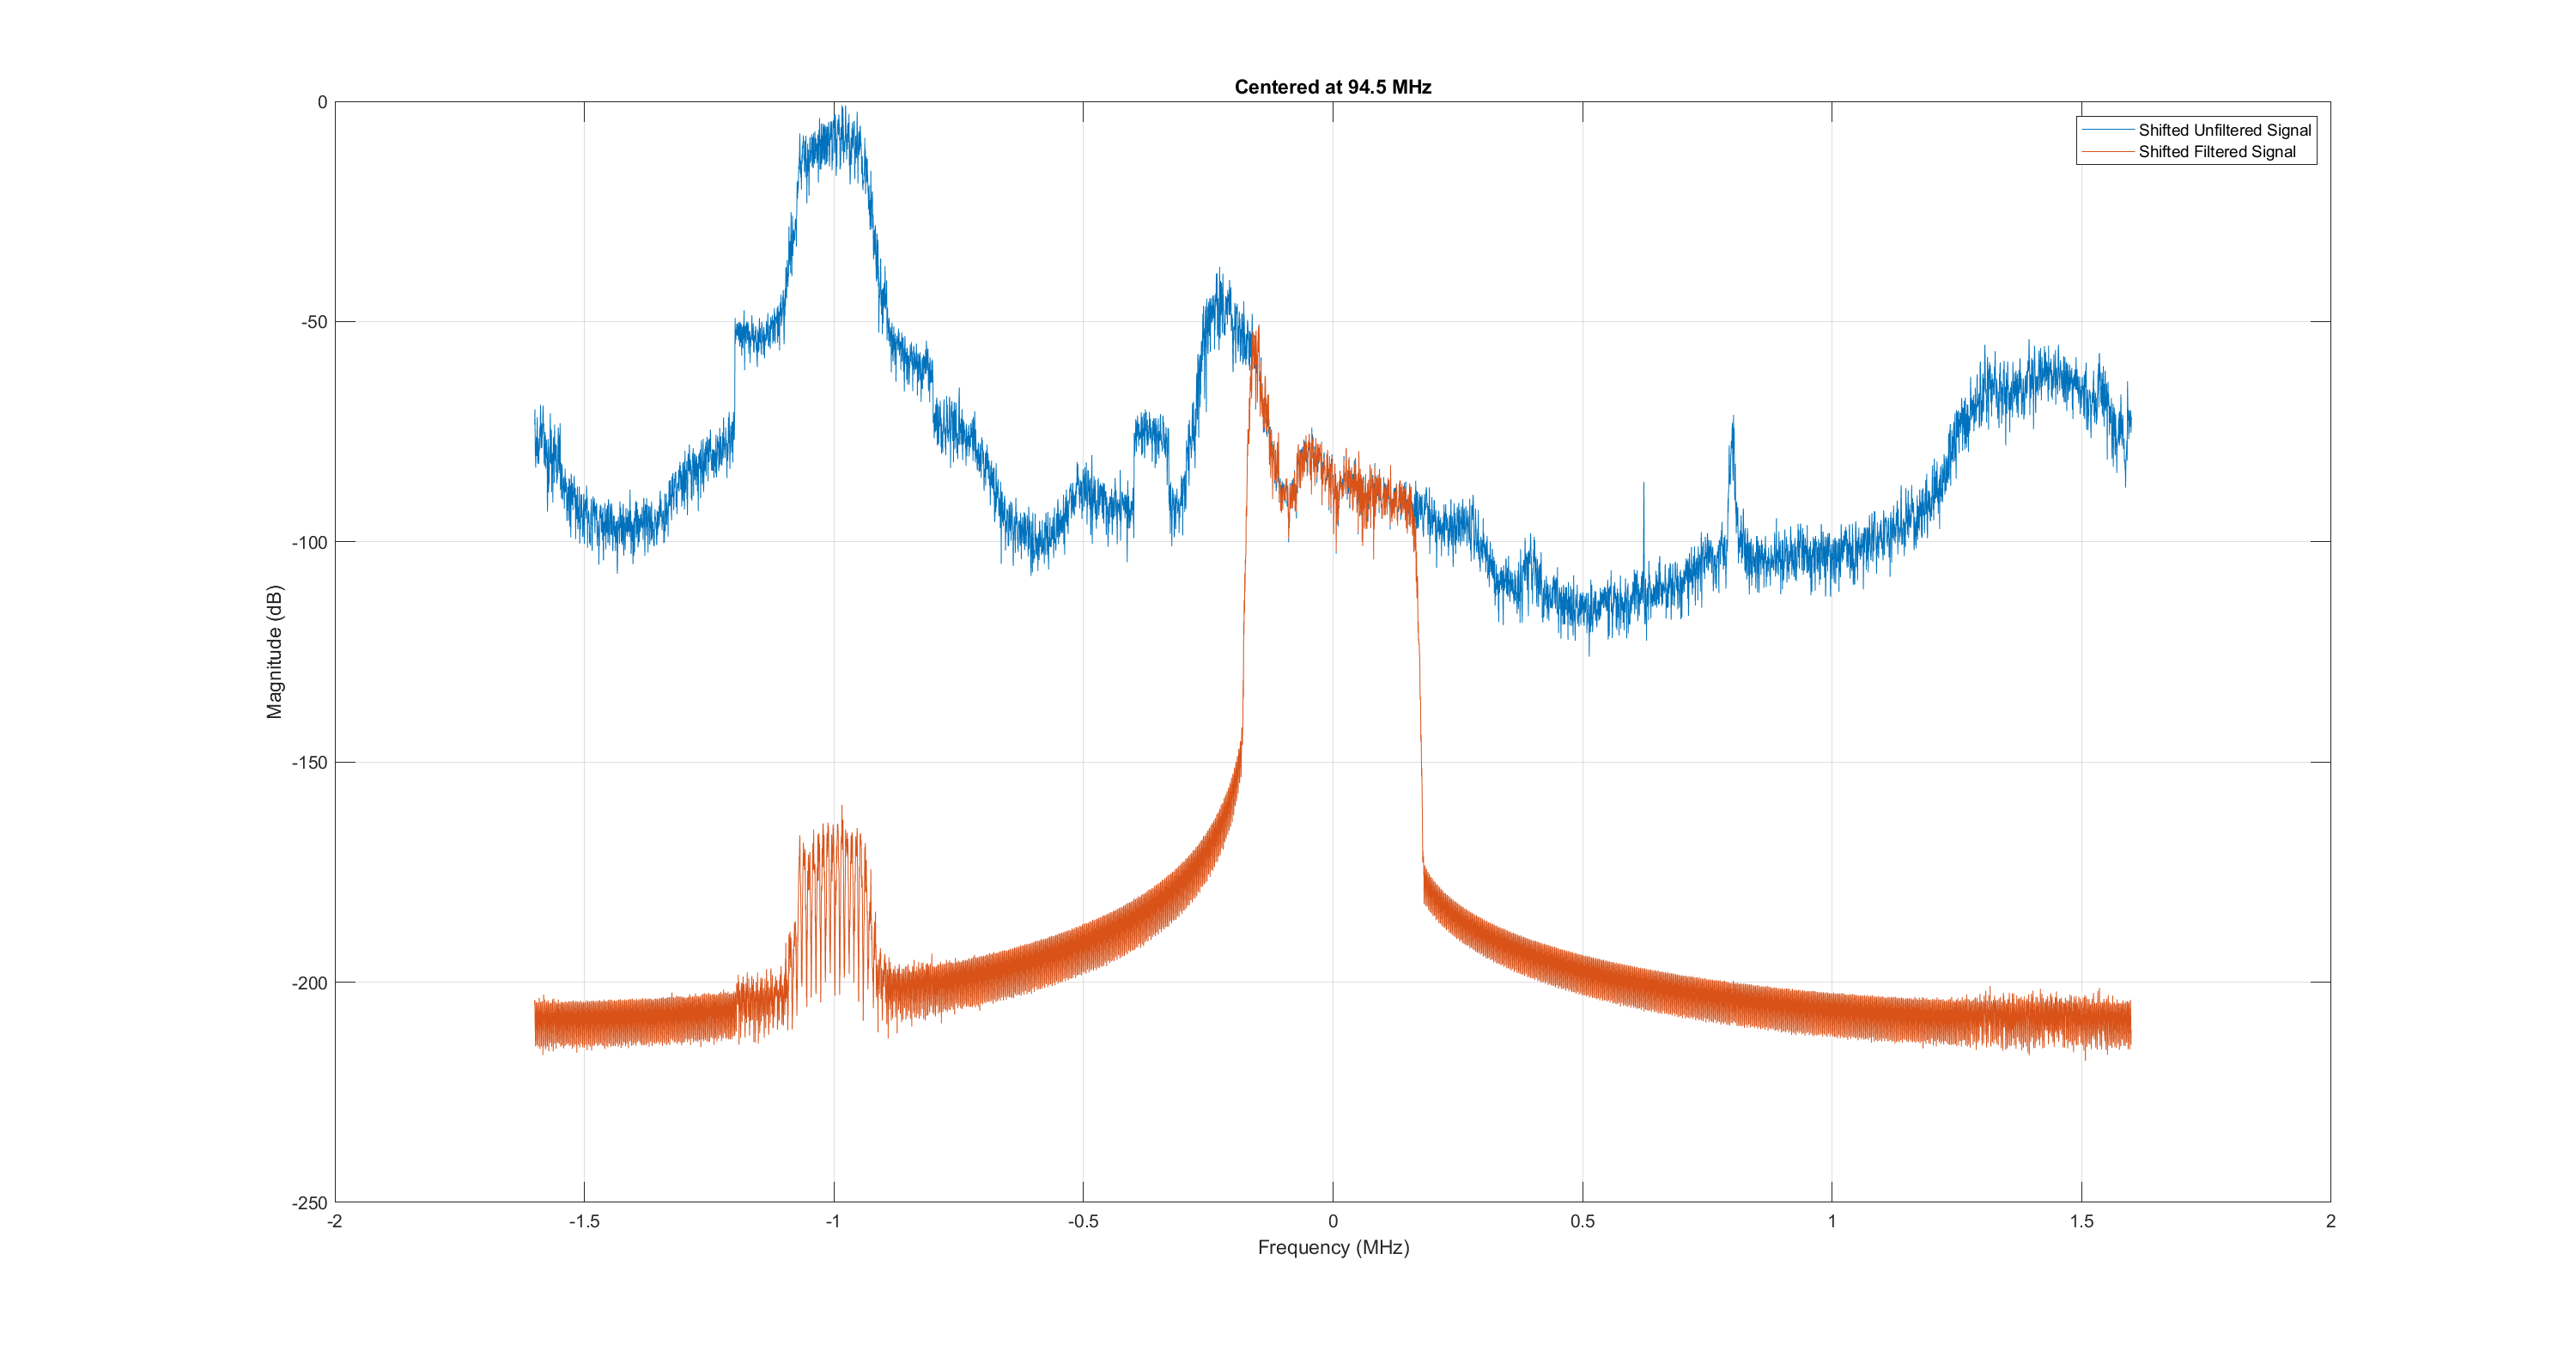
\includegraphics[width=\textwidth]{432_CA2_94.5.png}
        \caption{Centered at 94.5 MHz}
    \end{subfigure}
    \begin{subfigure}[b]{0.23\textwidth}
        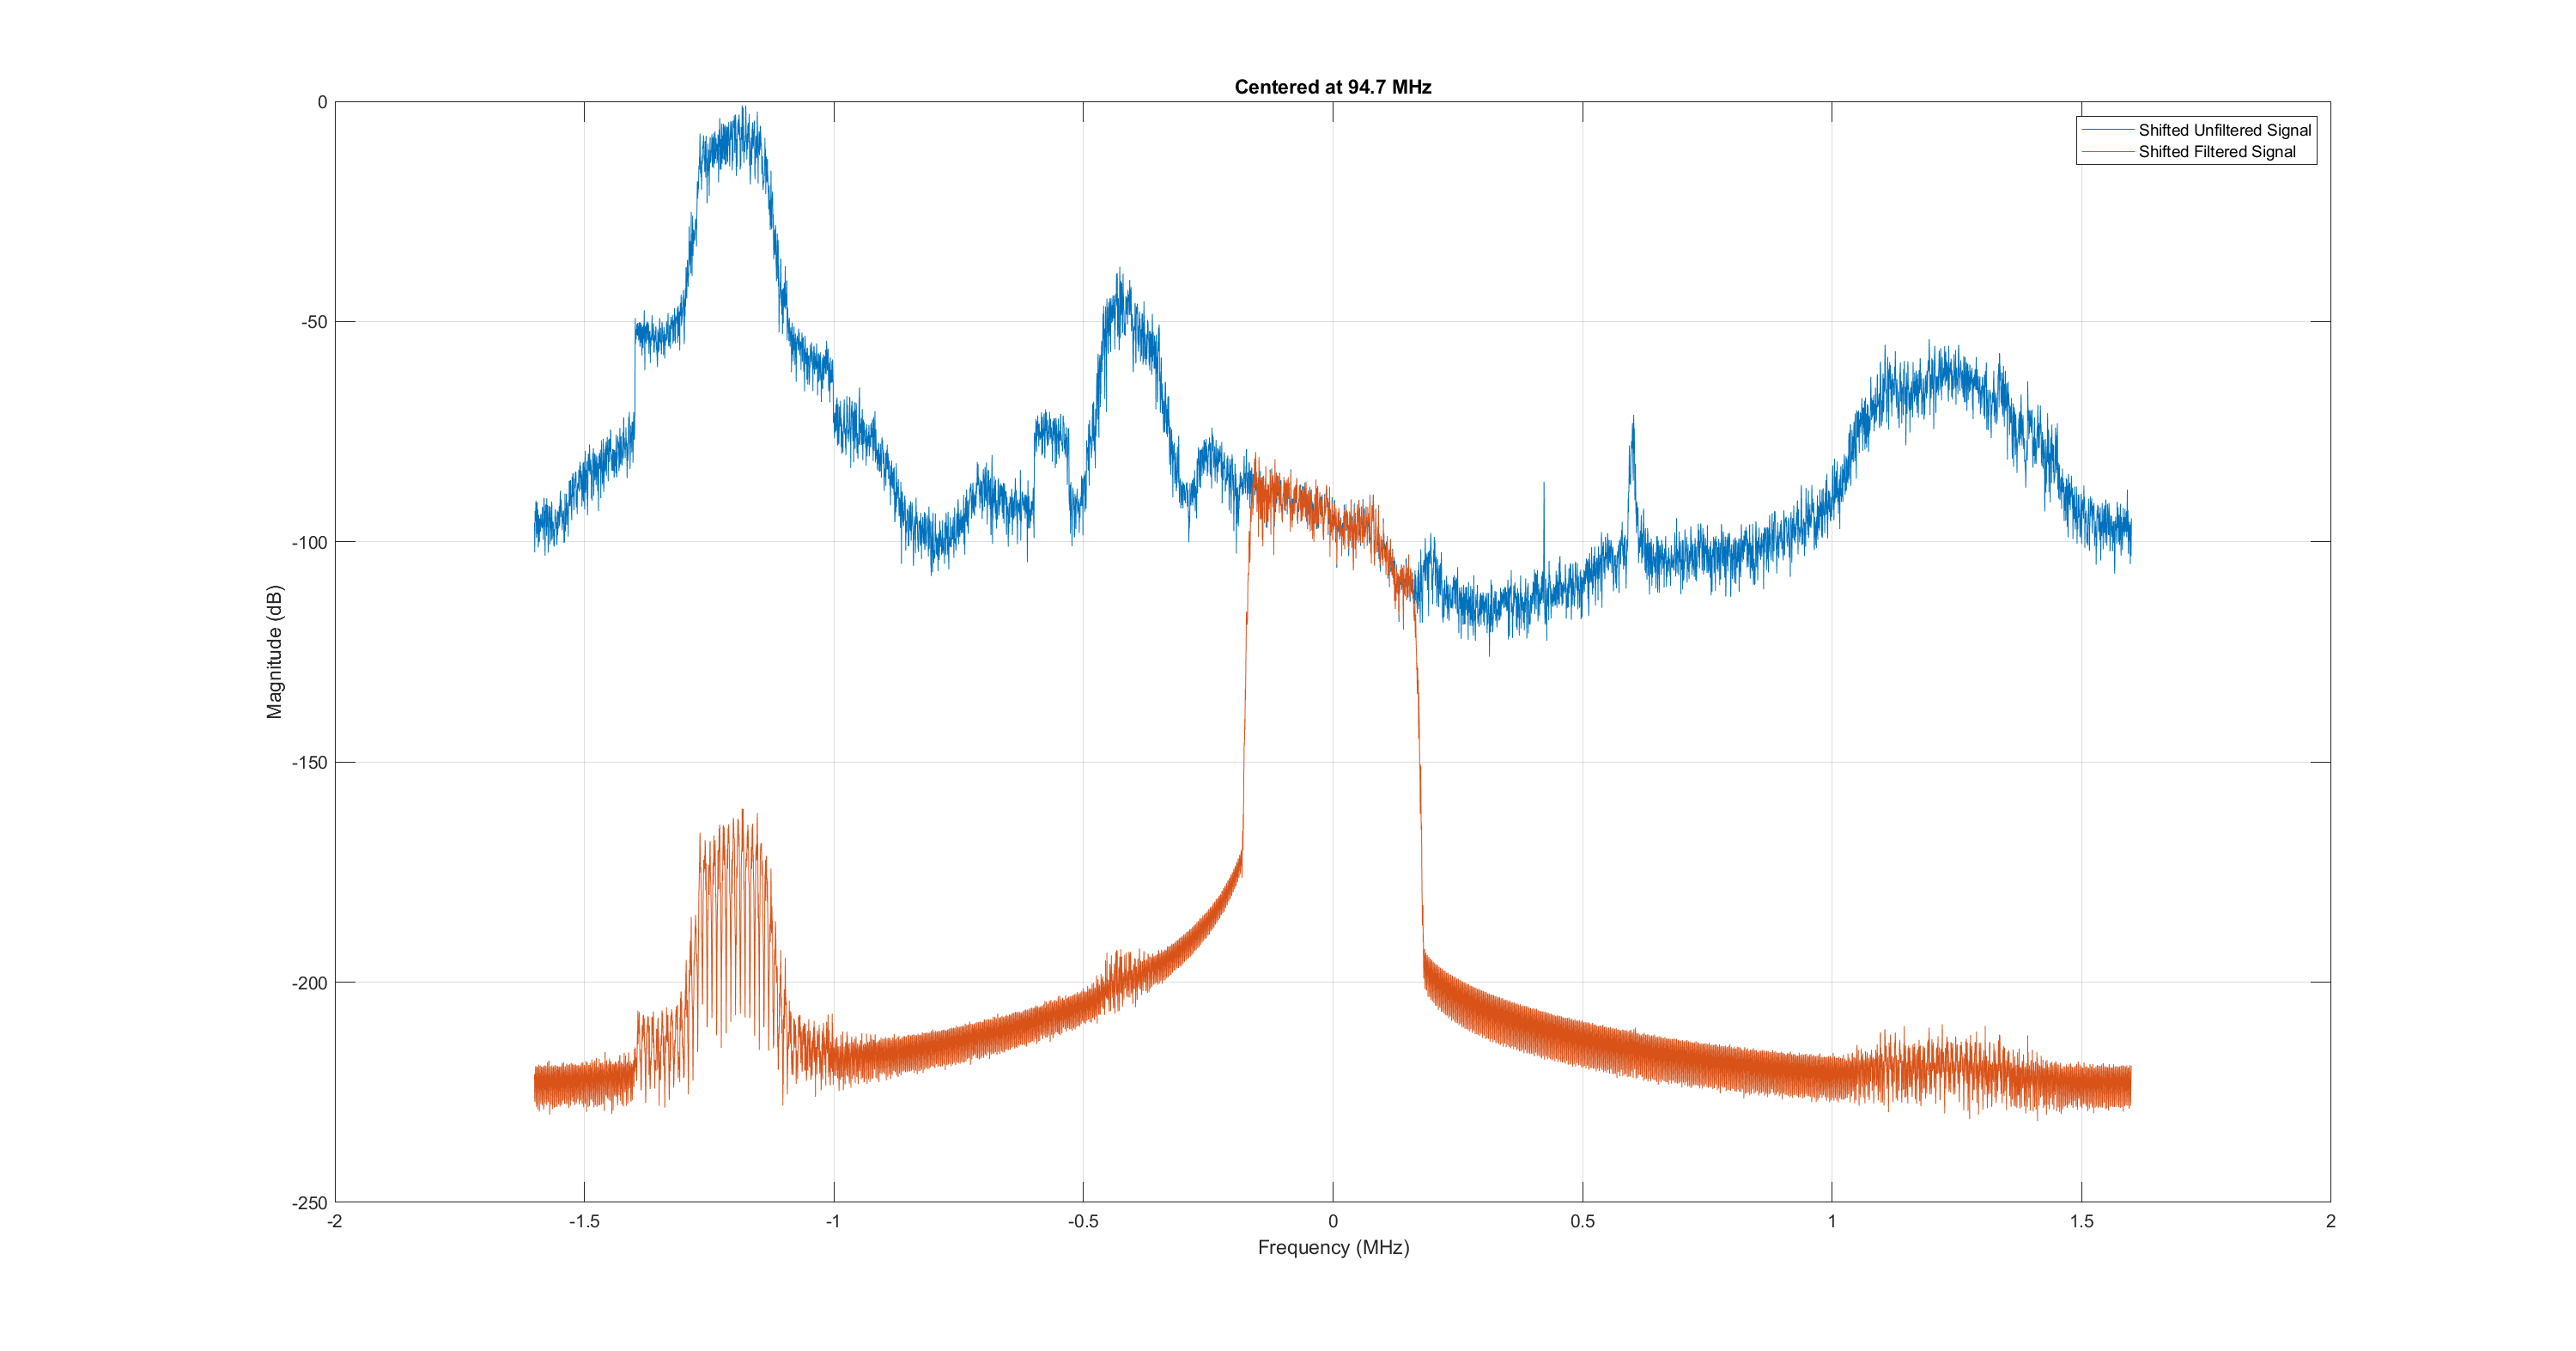
\includegraphics[width=\textwidth]{432_CA2_94.7.png}
        \caption{Centered at 94.7 MHz}
    \end{subfigure}
    \begin{subfigure}[b]{0.23\textwidth}
        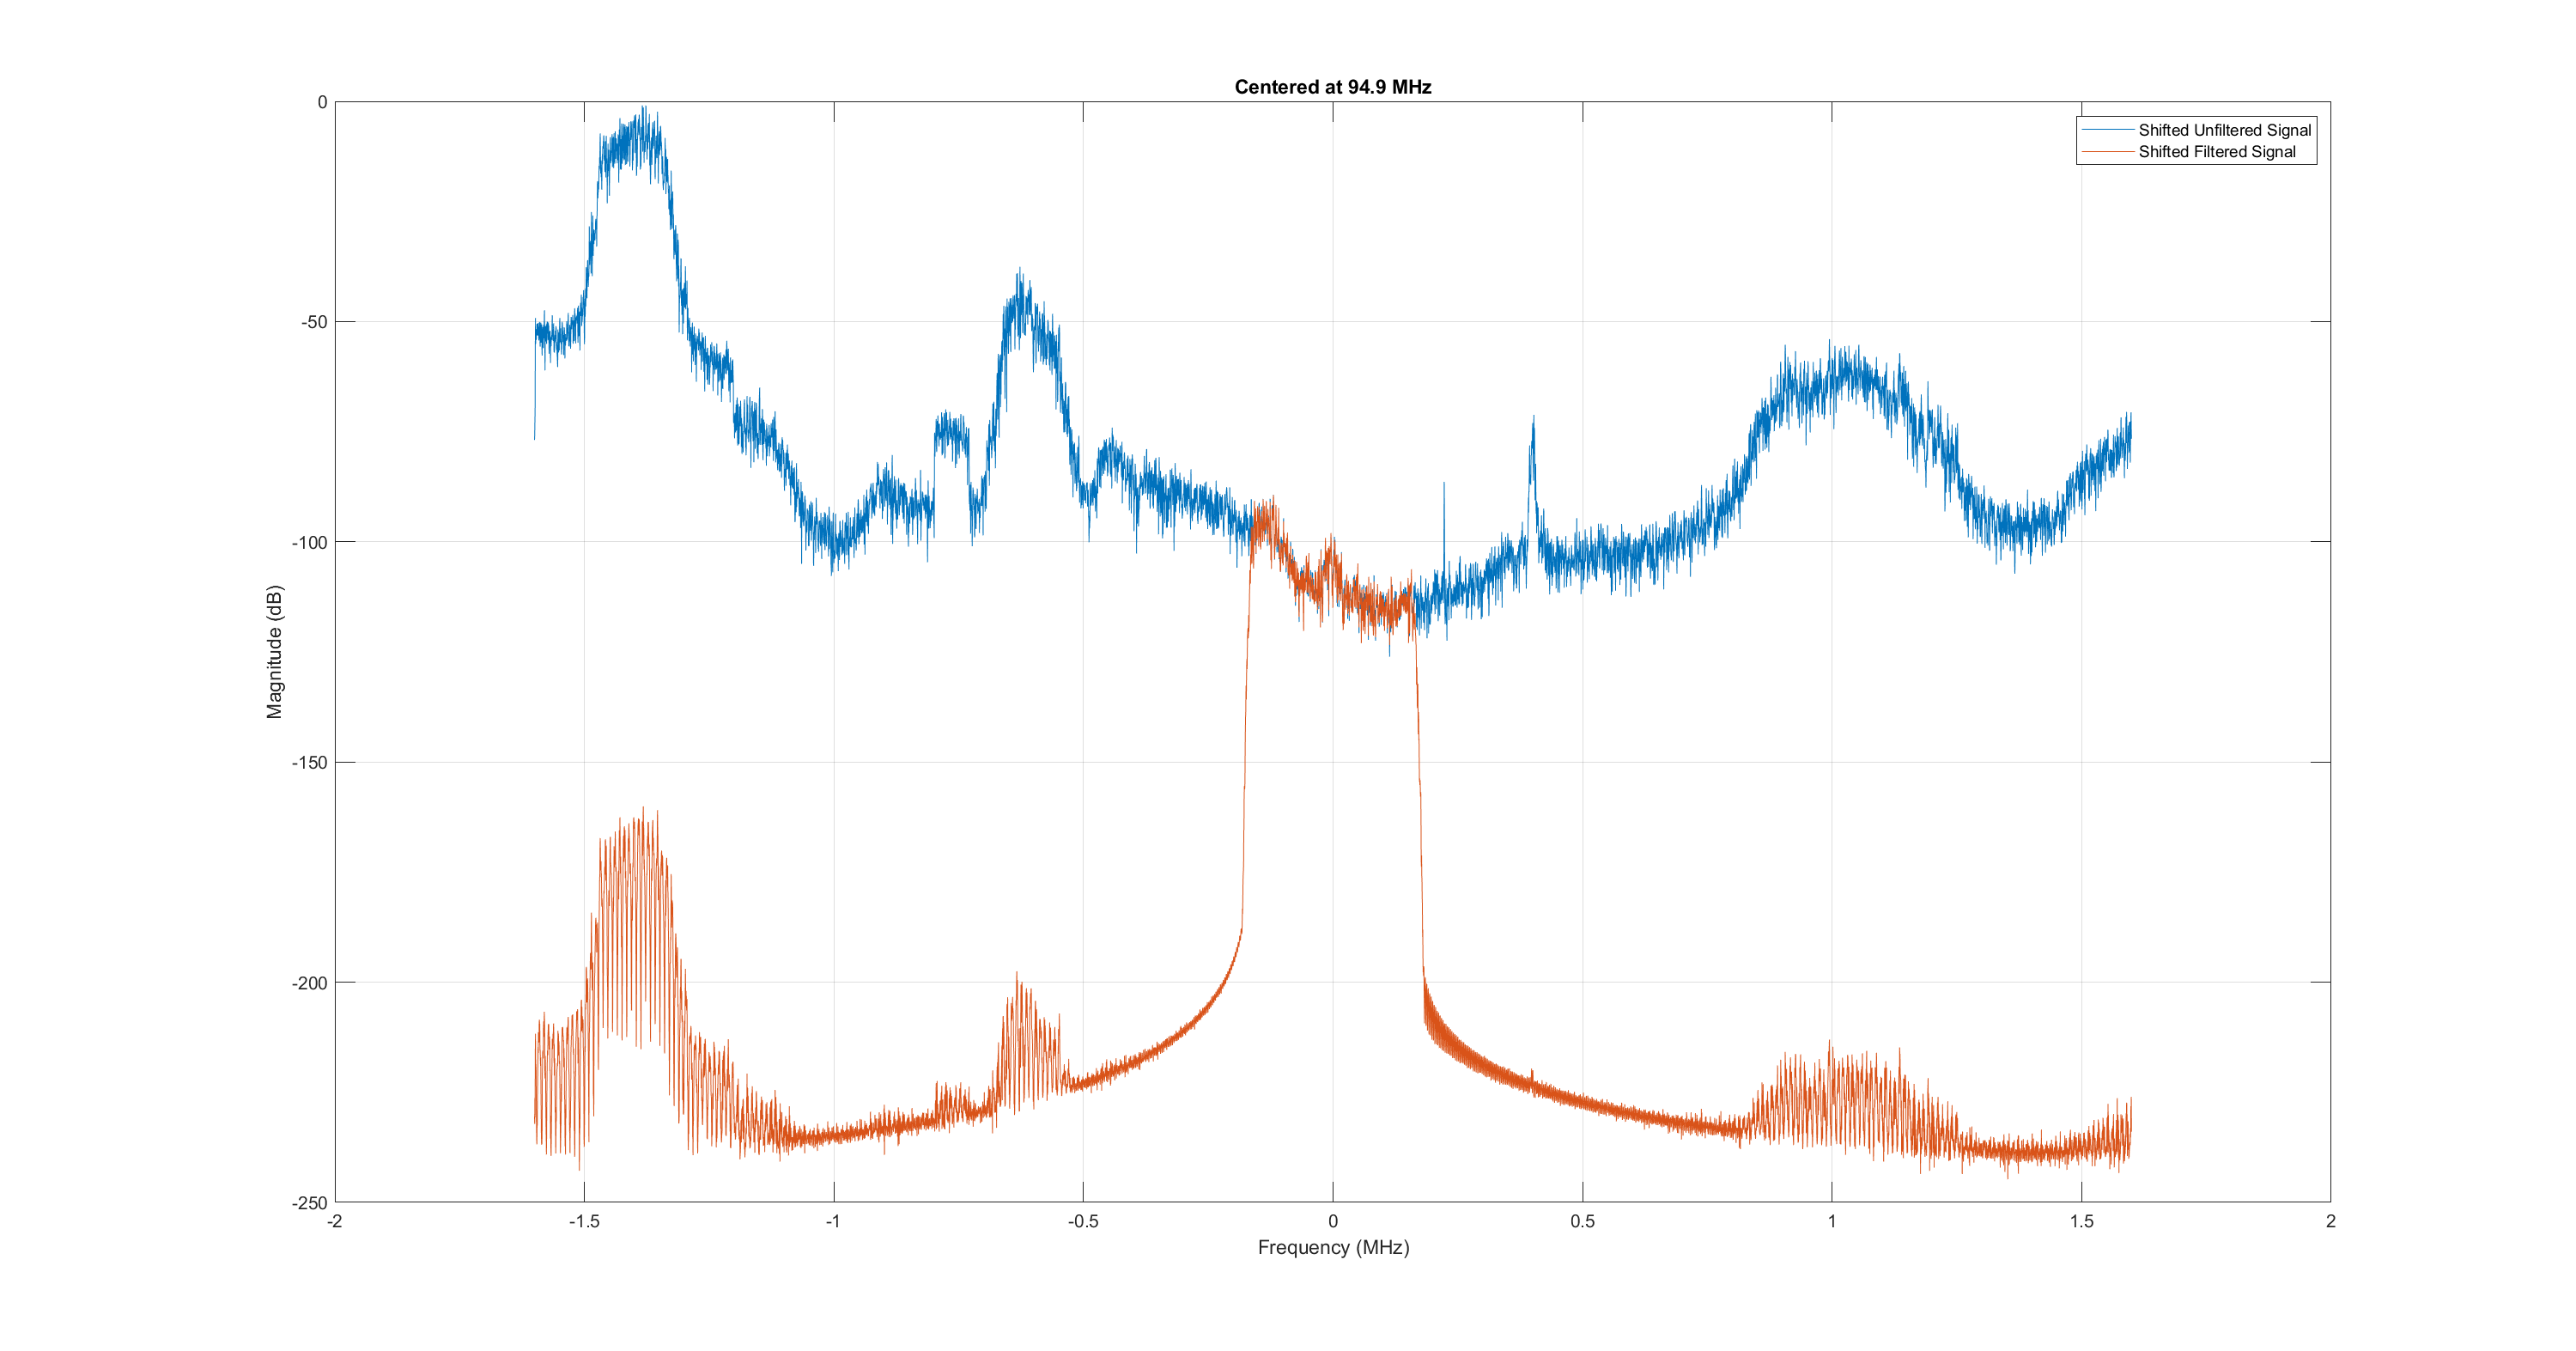
\includegraphics[width=\textwidth]{432_CA2_94.9.png}
        \caption{Centered at 94.9 MHz}
    \end{subfigure}
    \begin{subfigure}[b]{0.23\textwidth}
        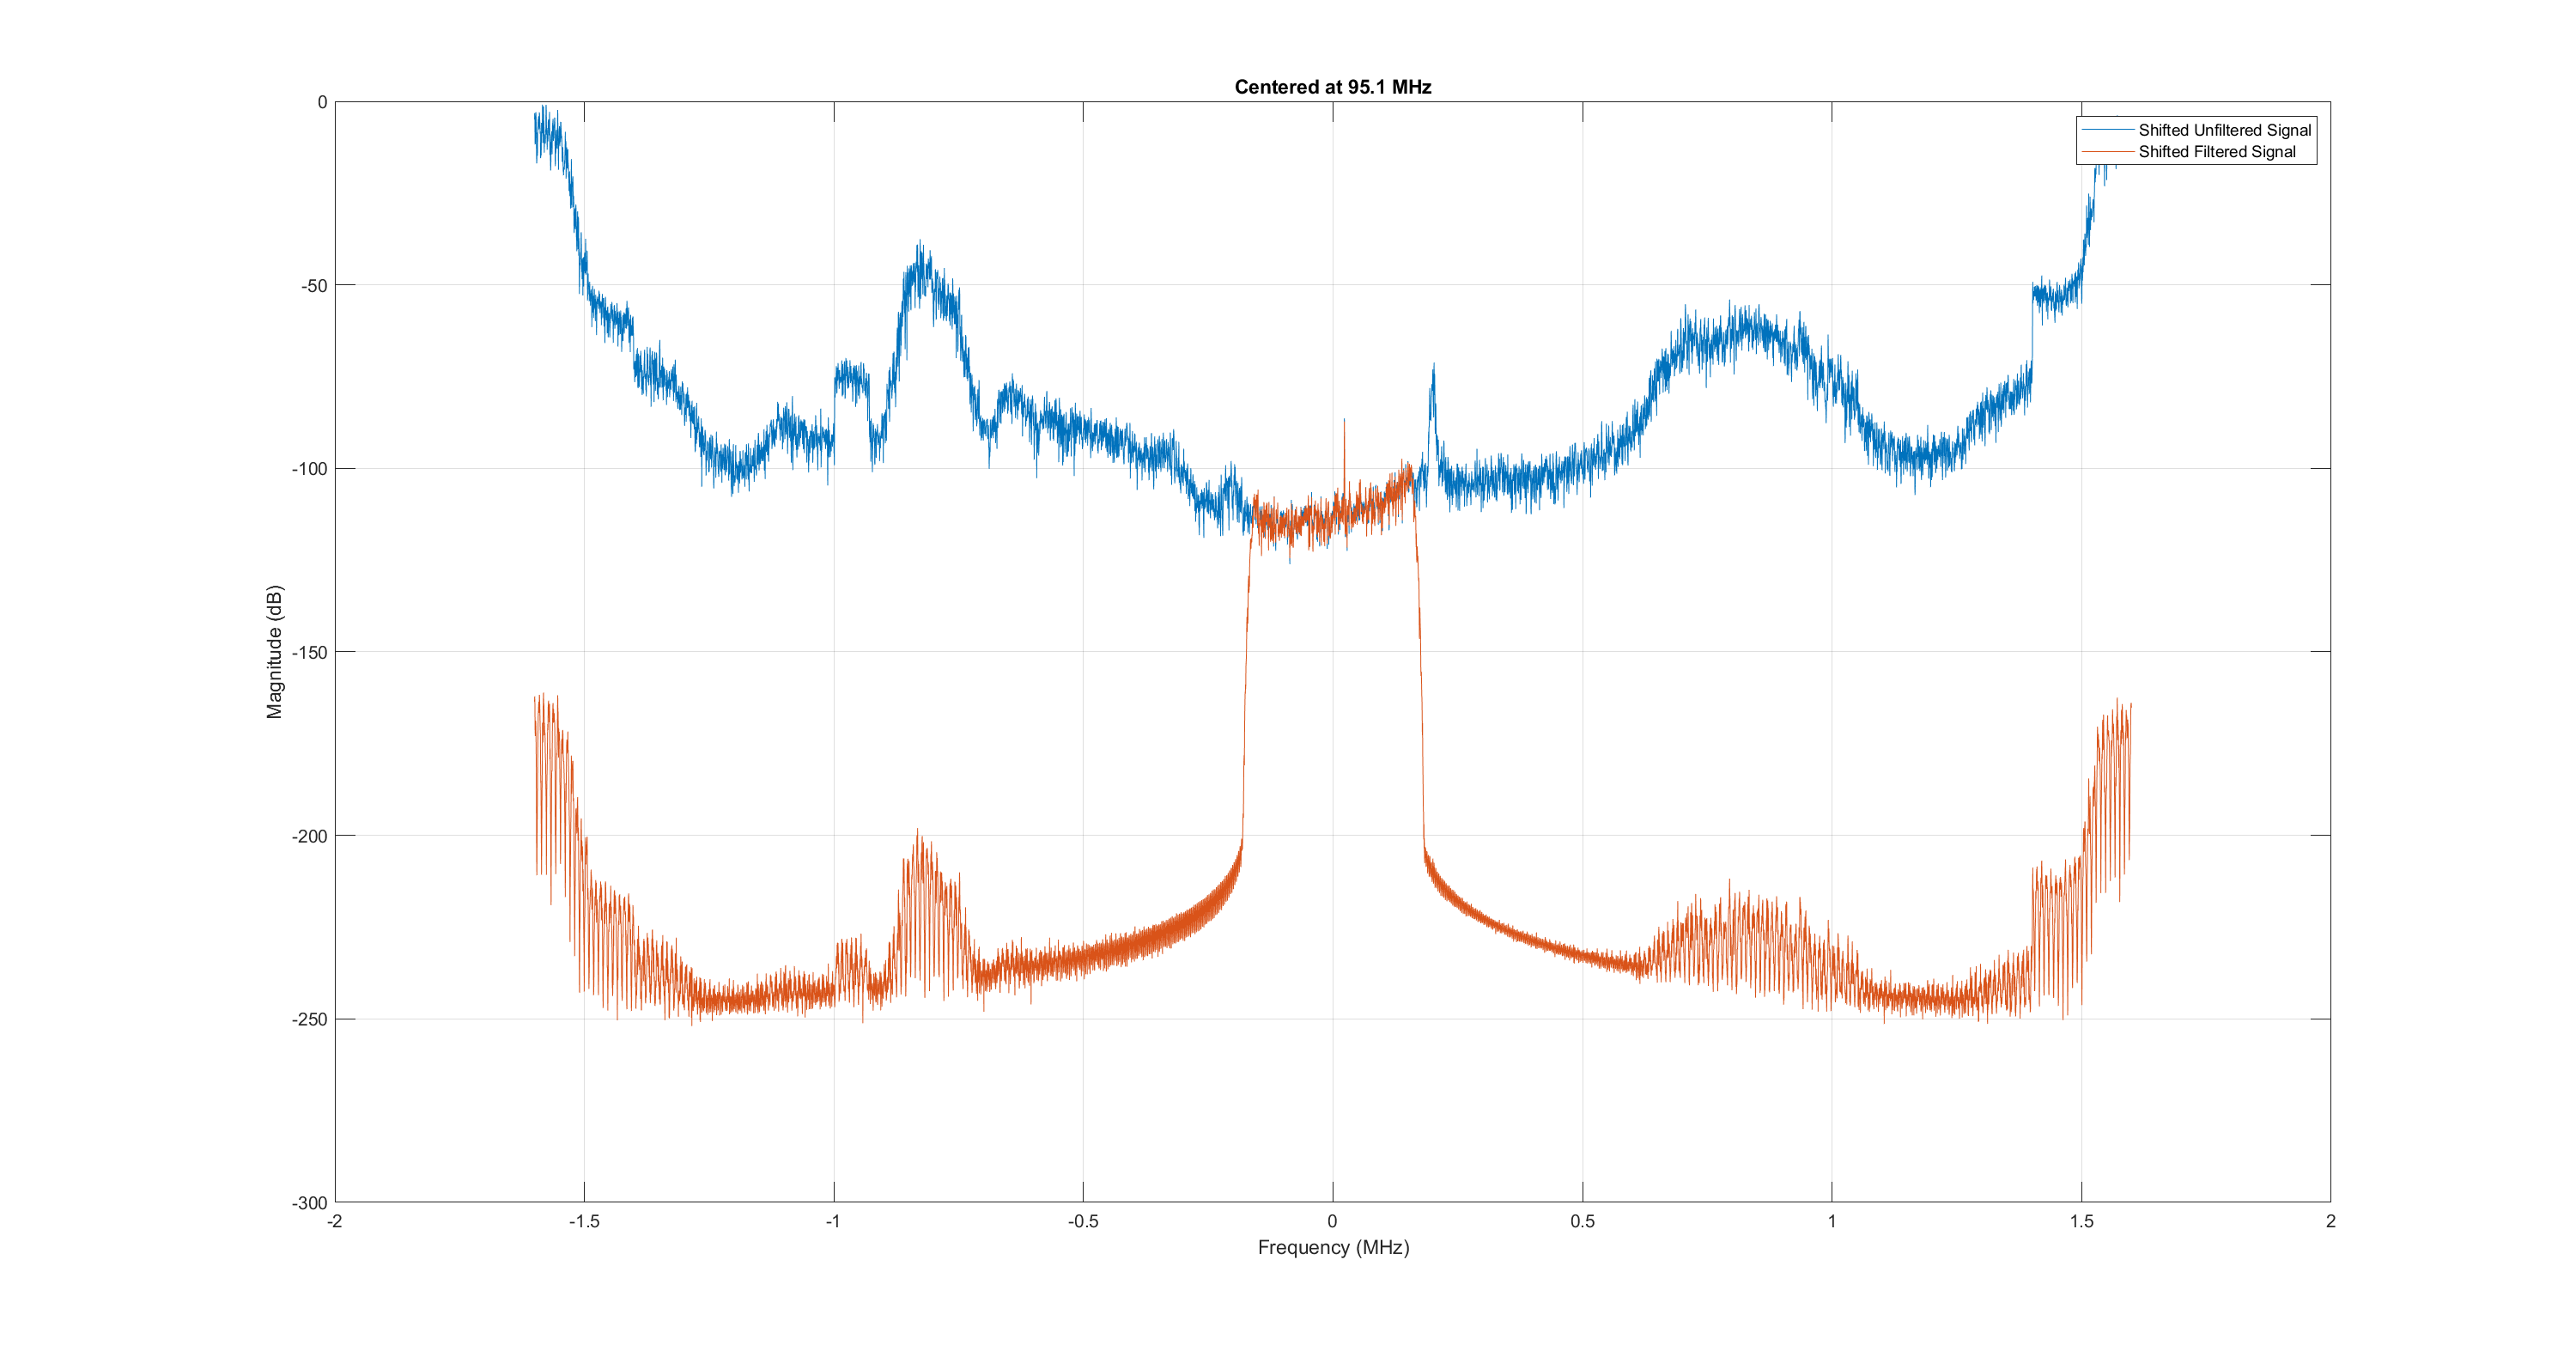
\includegraphics[width=\textwidth]{432_CA2_95.1.png}
        \caption{Centered at 95.1 MHz}
    \end{subfigure}
    
    % Row 2
    \begin{subfigure}[b]{0.23\textwidth}
        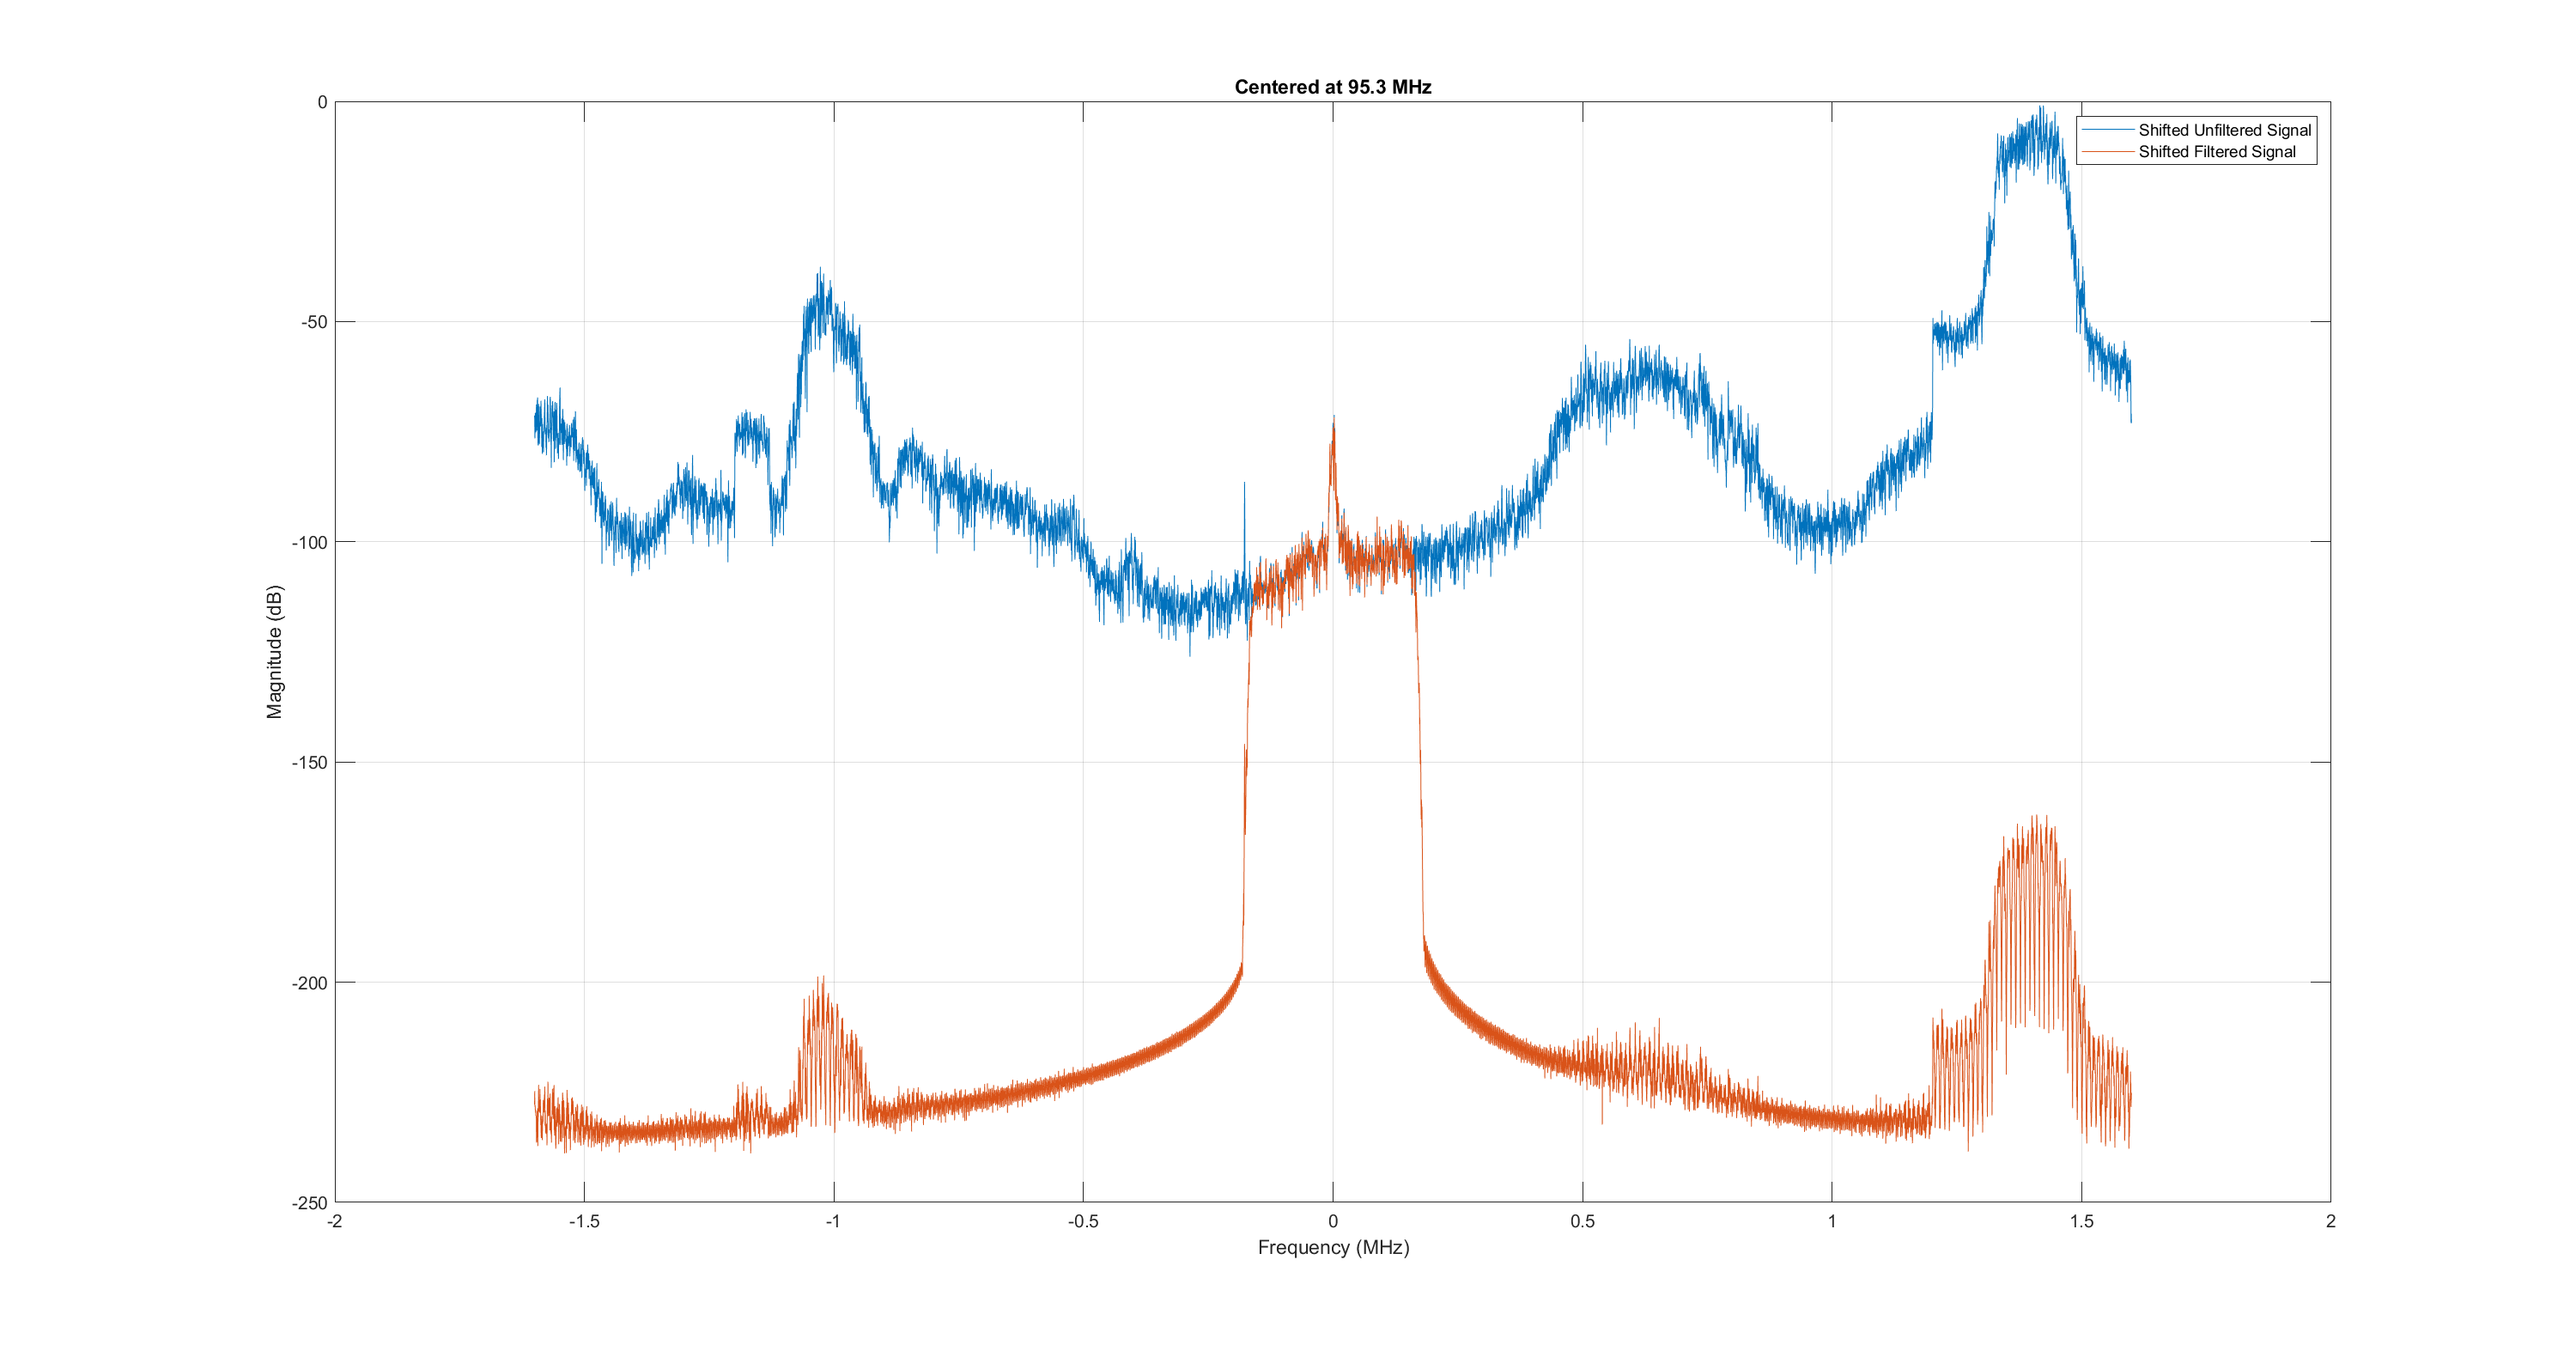
\includegraphics[width=\textwidth]{432_CA2_95.3.png}
        \caption{Centered at 95.3 MHz}
    \end{subfigure}
    \begin{subfigure}[b]{0.23\textwidth}
        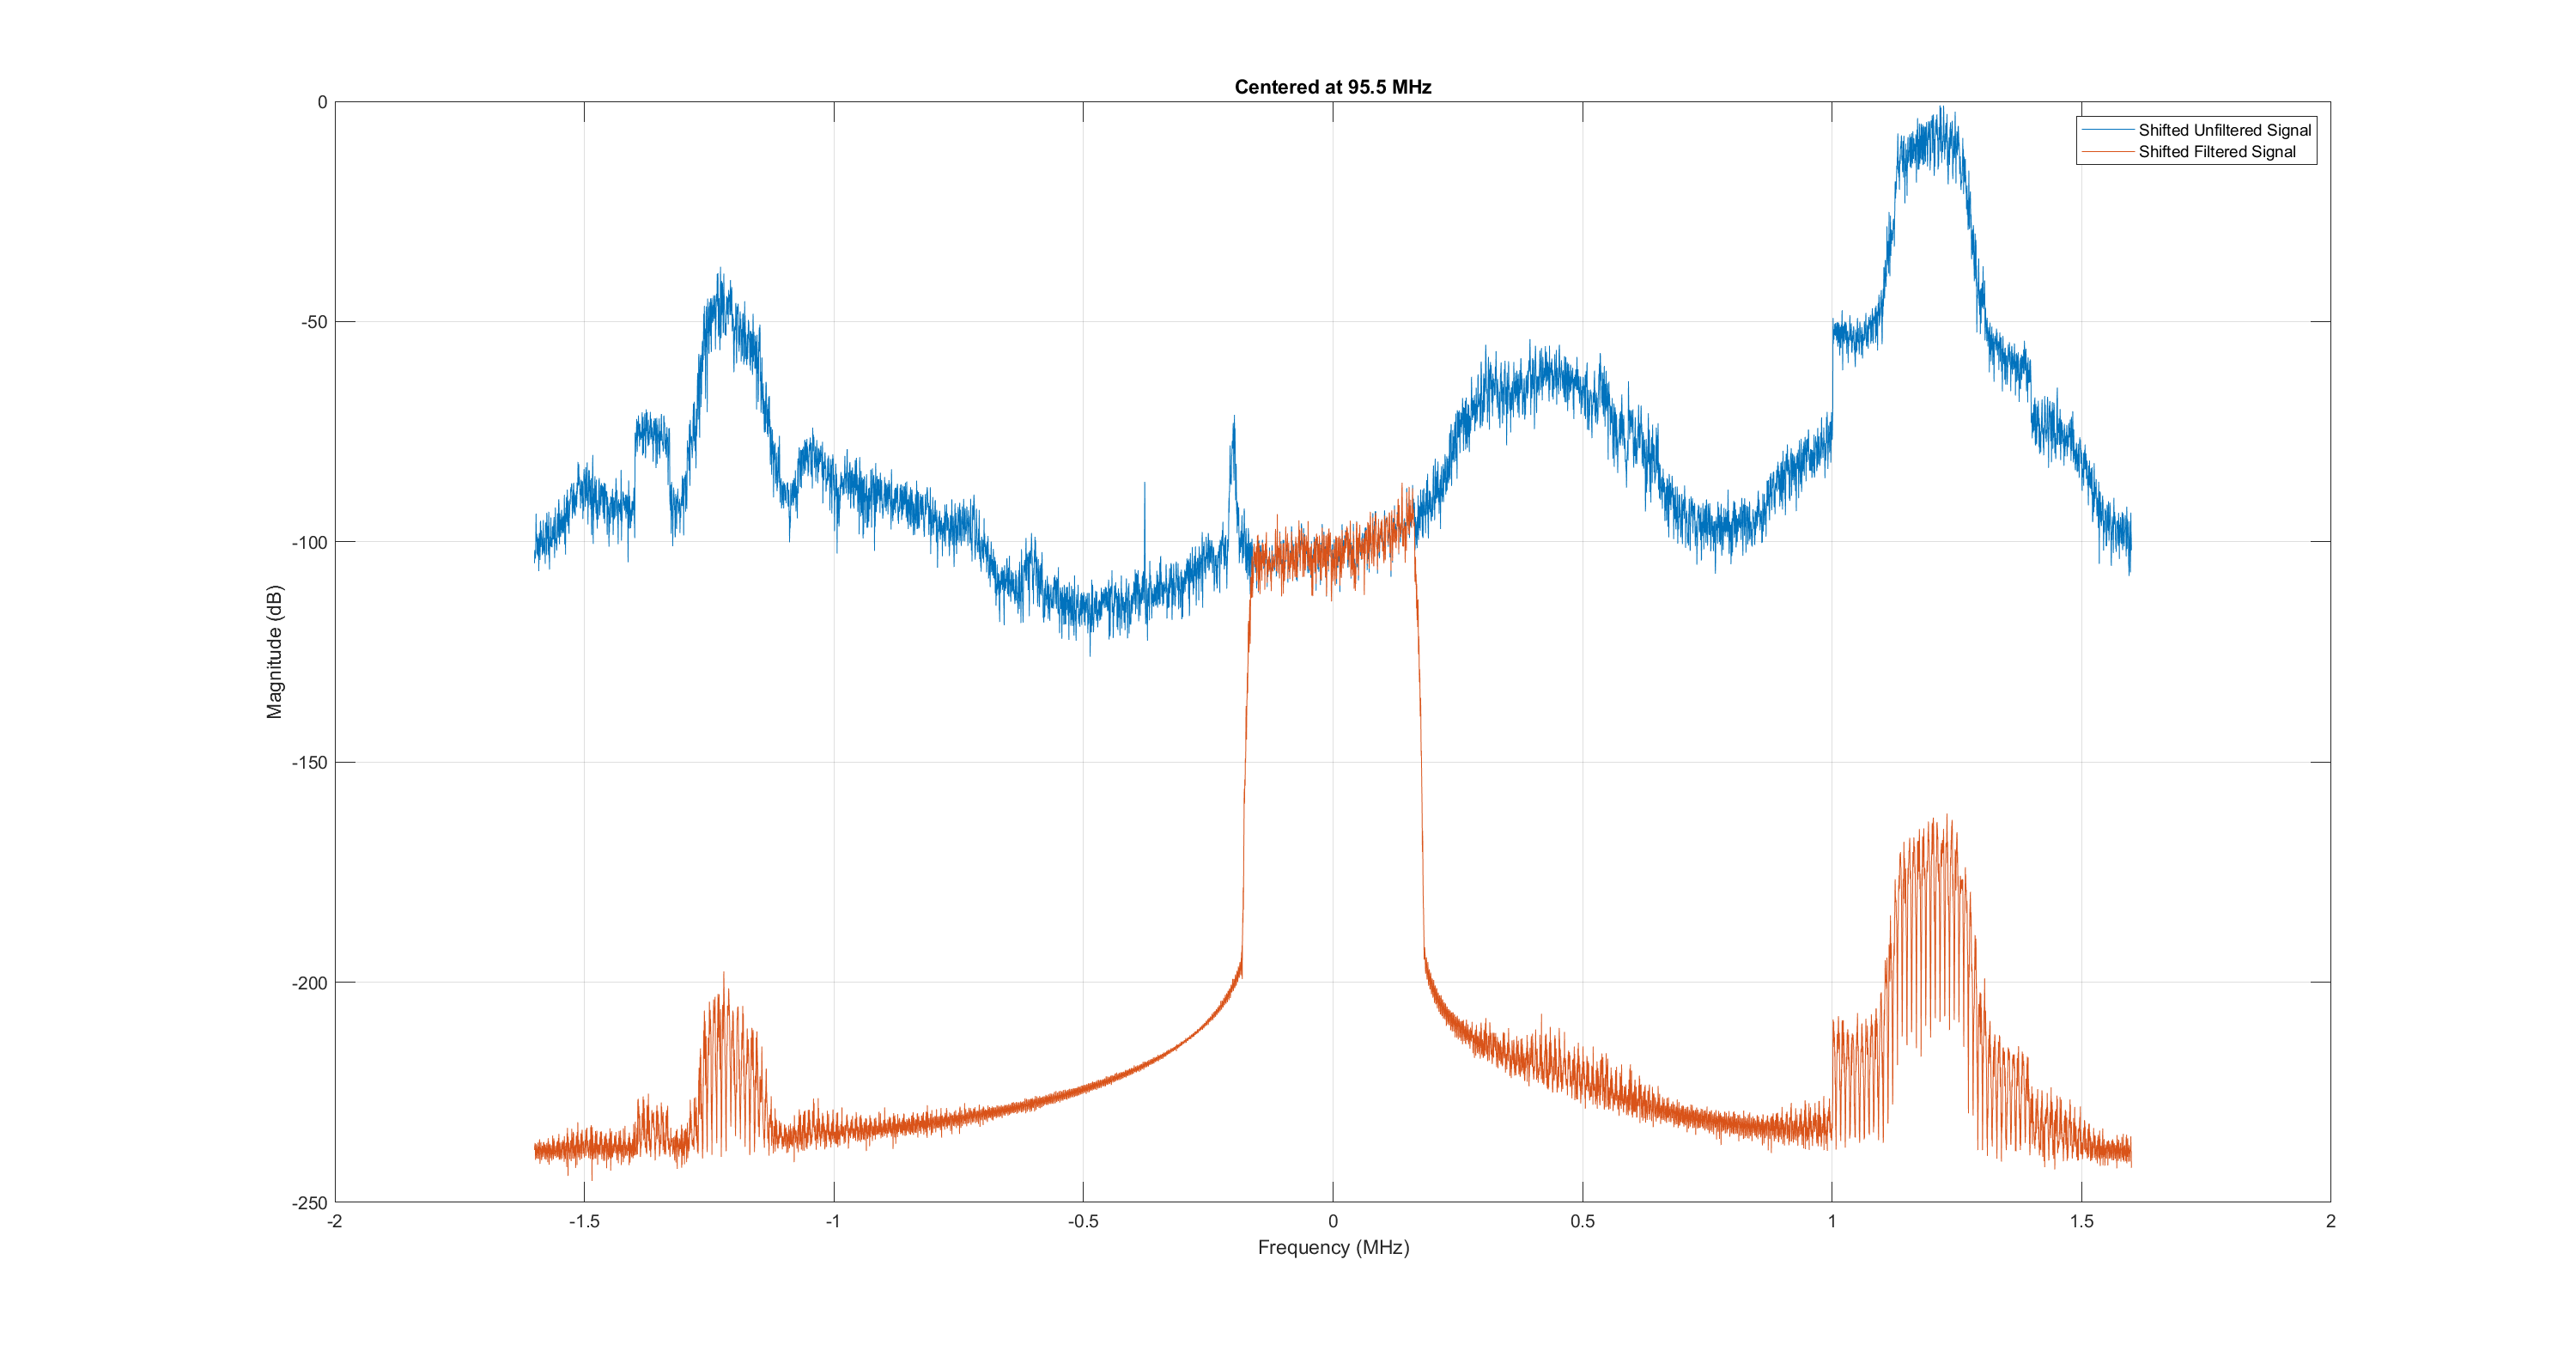
\includegraphics[width=\textwidth]{432_CA2_95.5.png}
        \caption{Centered at 95.5 MHz}
    \end{subfigure}
    \begin{subfigure}[b]{0.23\textwidth}
        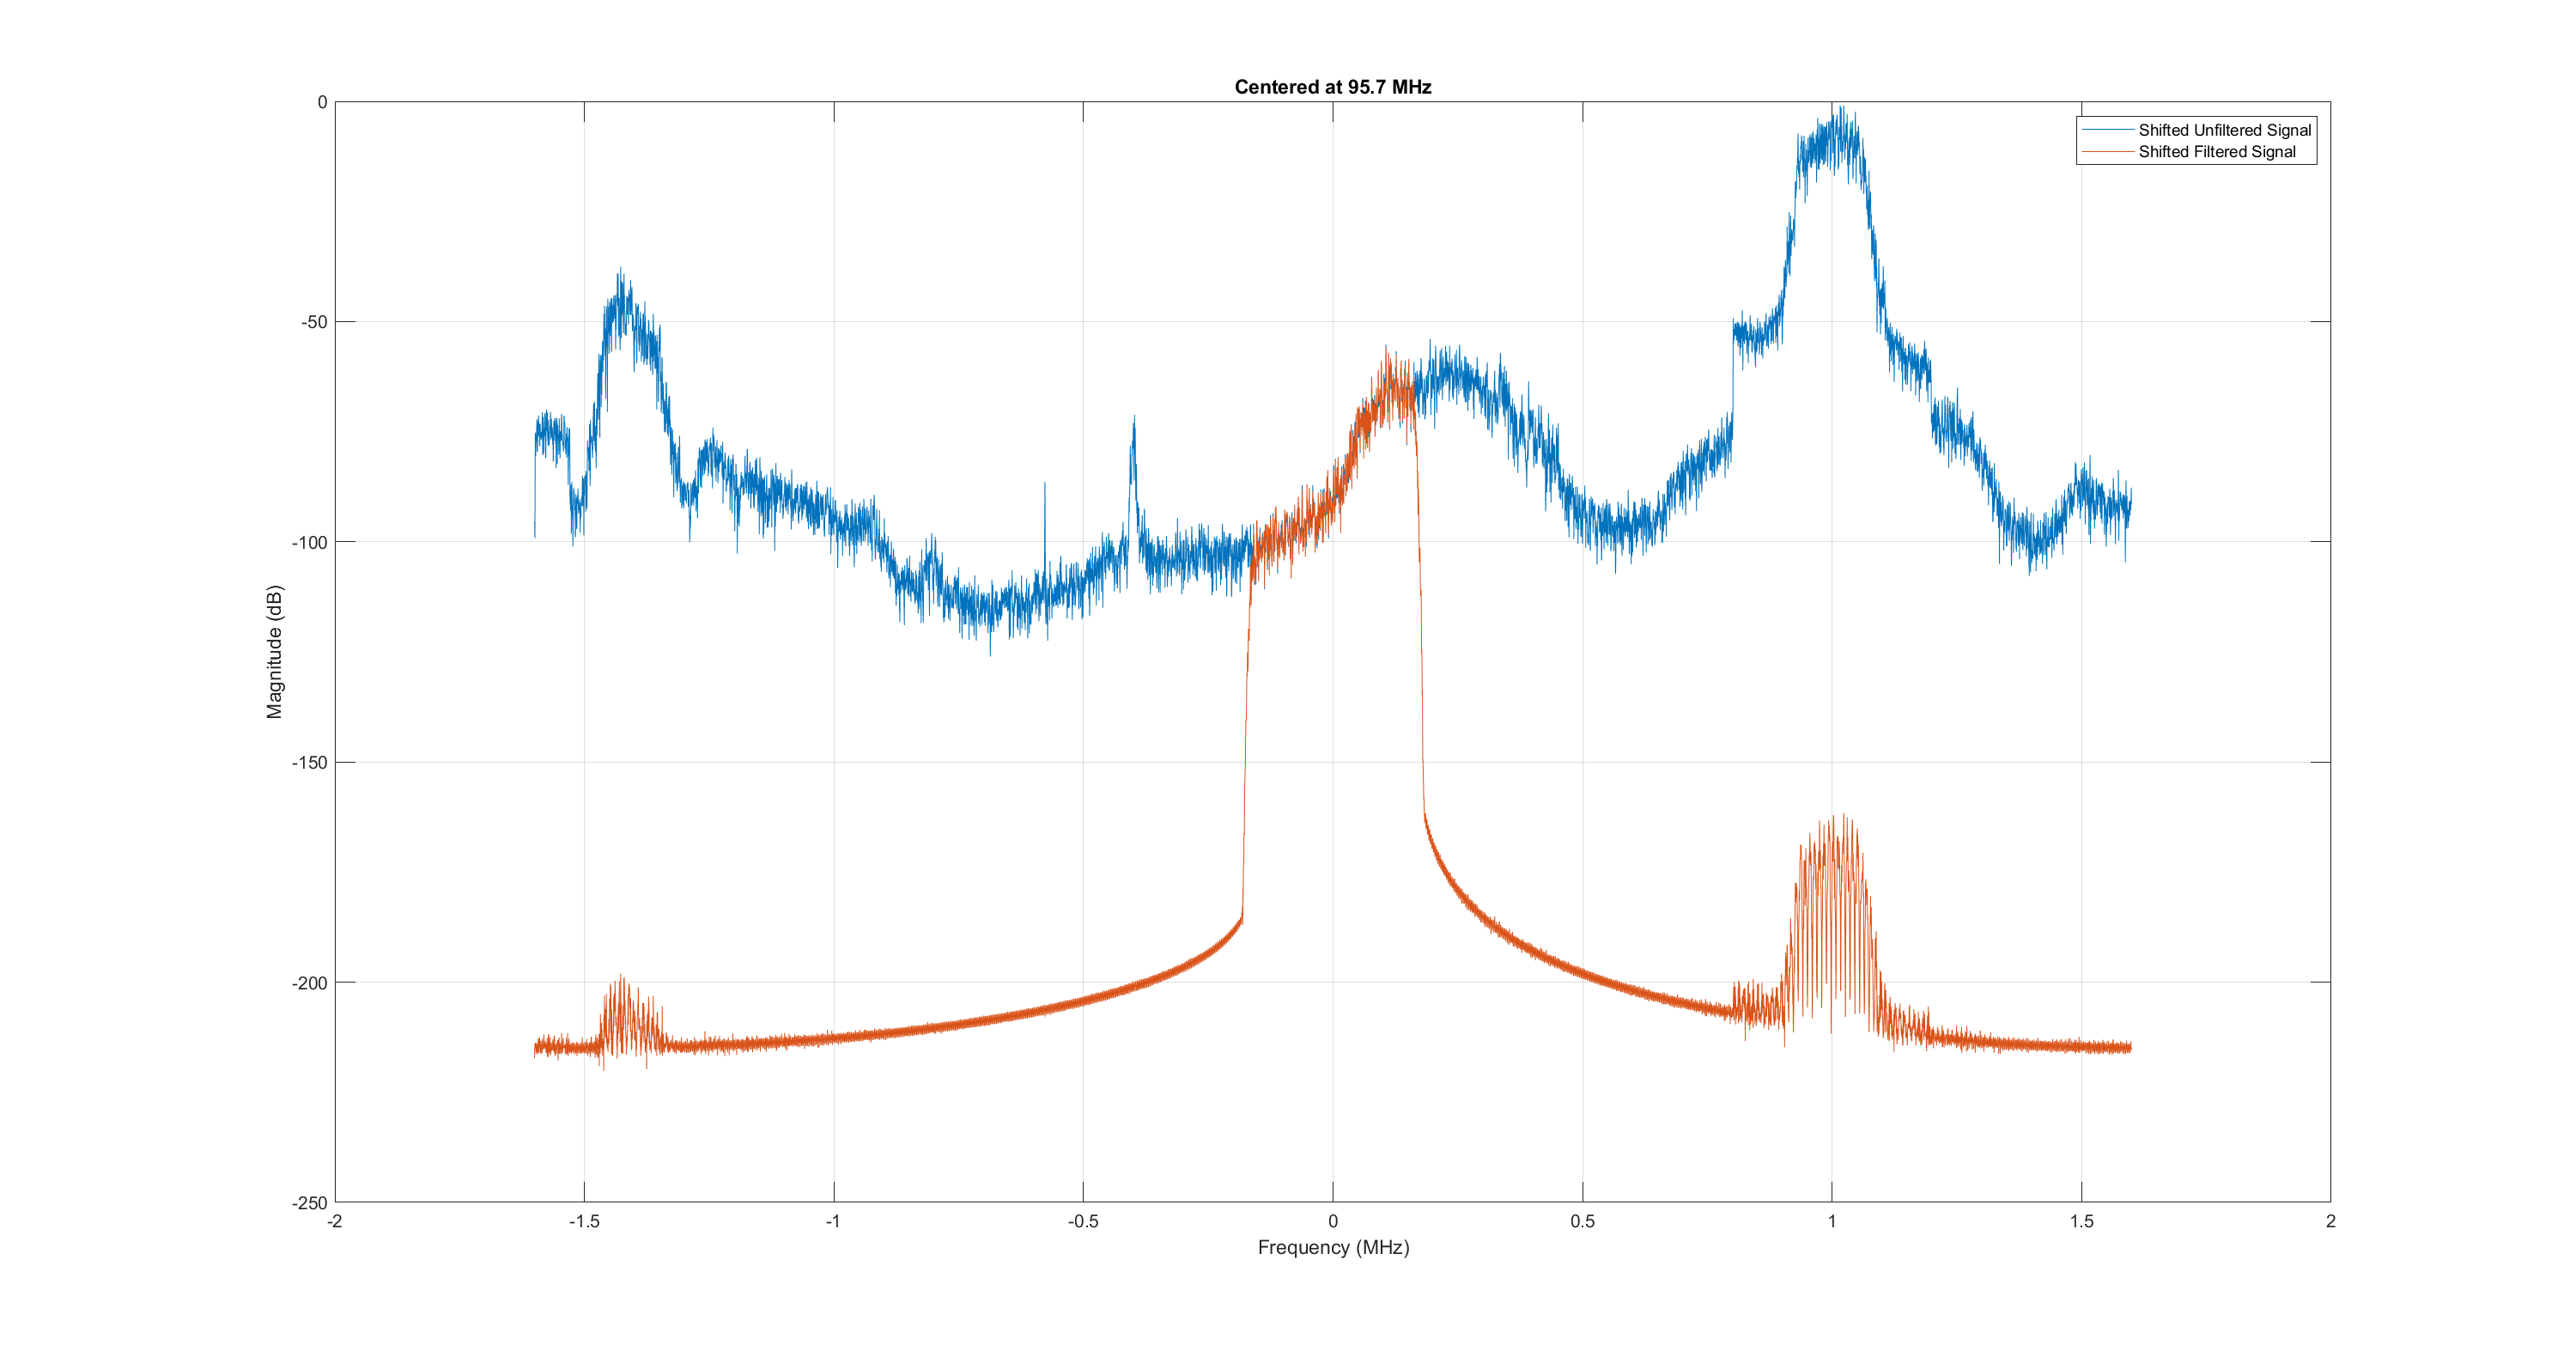
\includegraphics[width=\textwidth]{432_CA2_95.7.png}
        \caption{Centered at 95.7 MHz}
    \end{subfigure}
    \begin{subfigure}[b]{0.23\textwidth}
        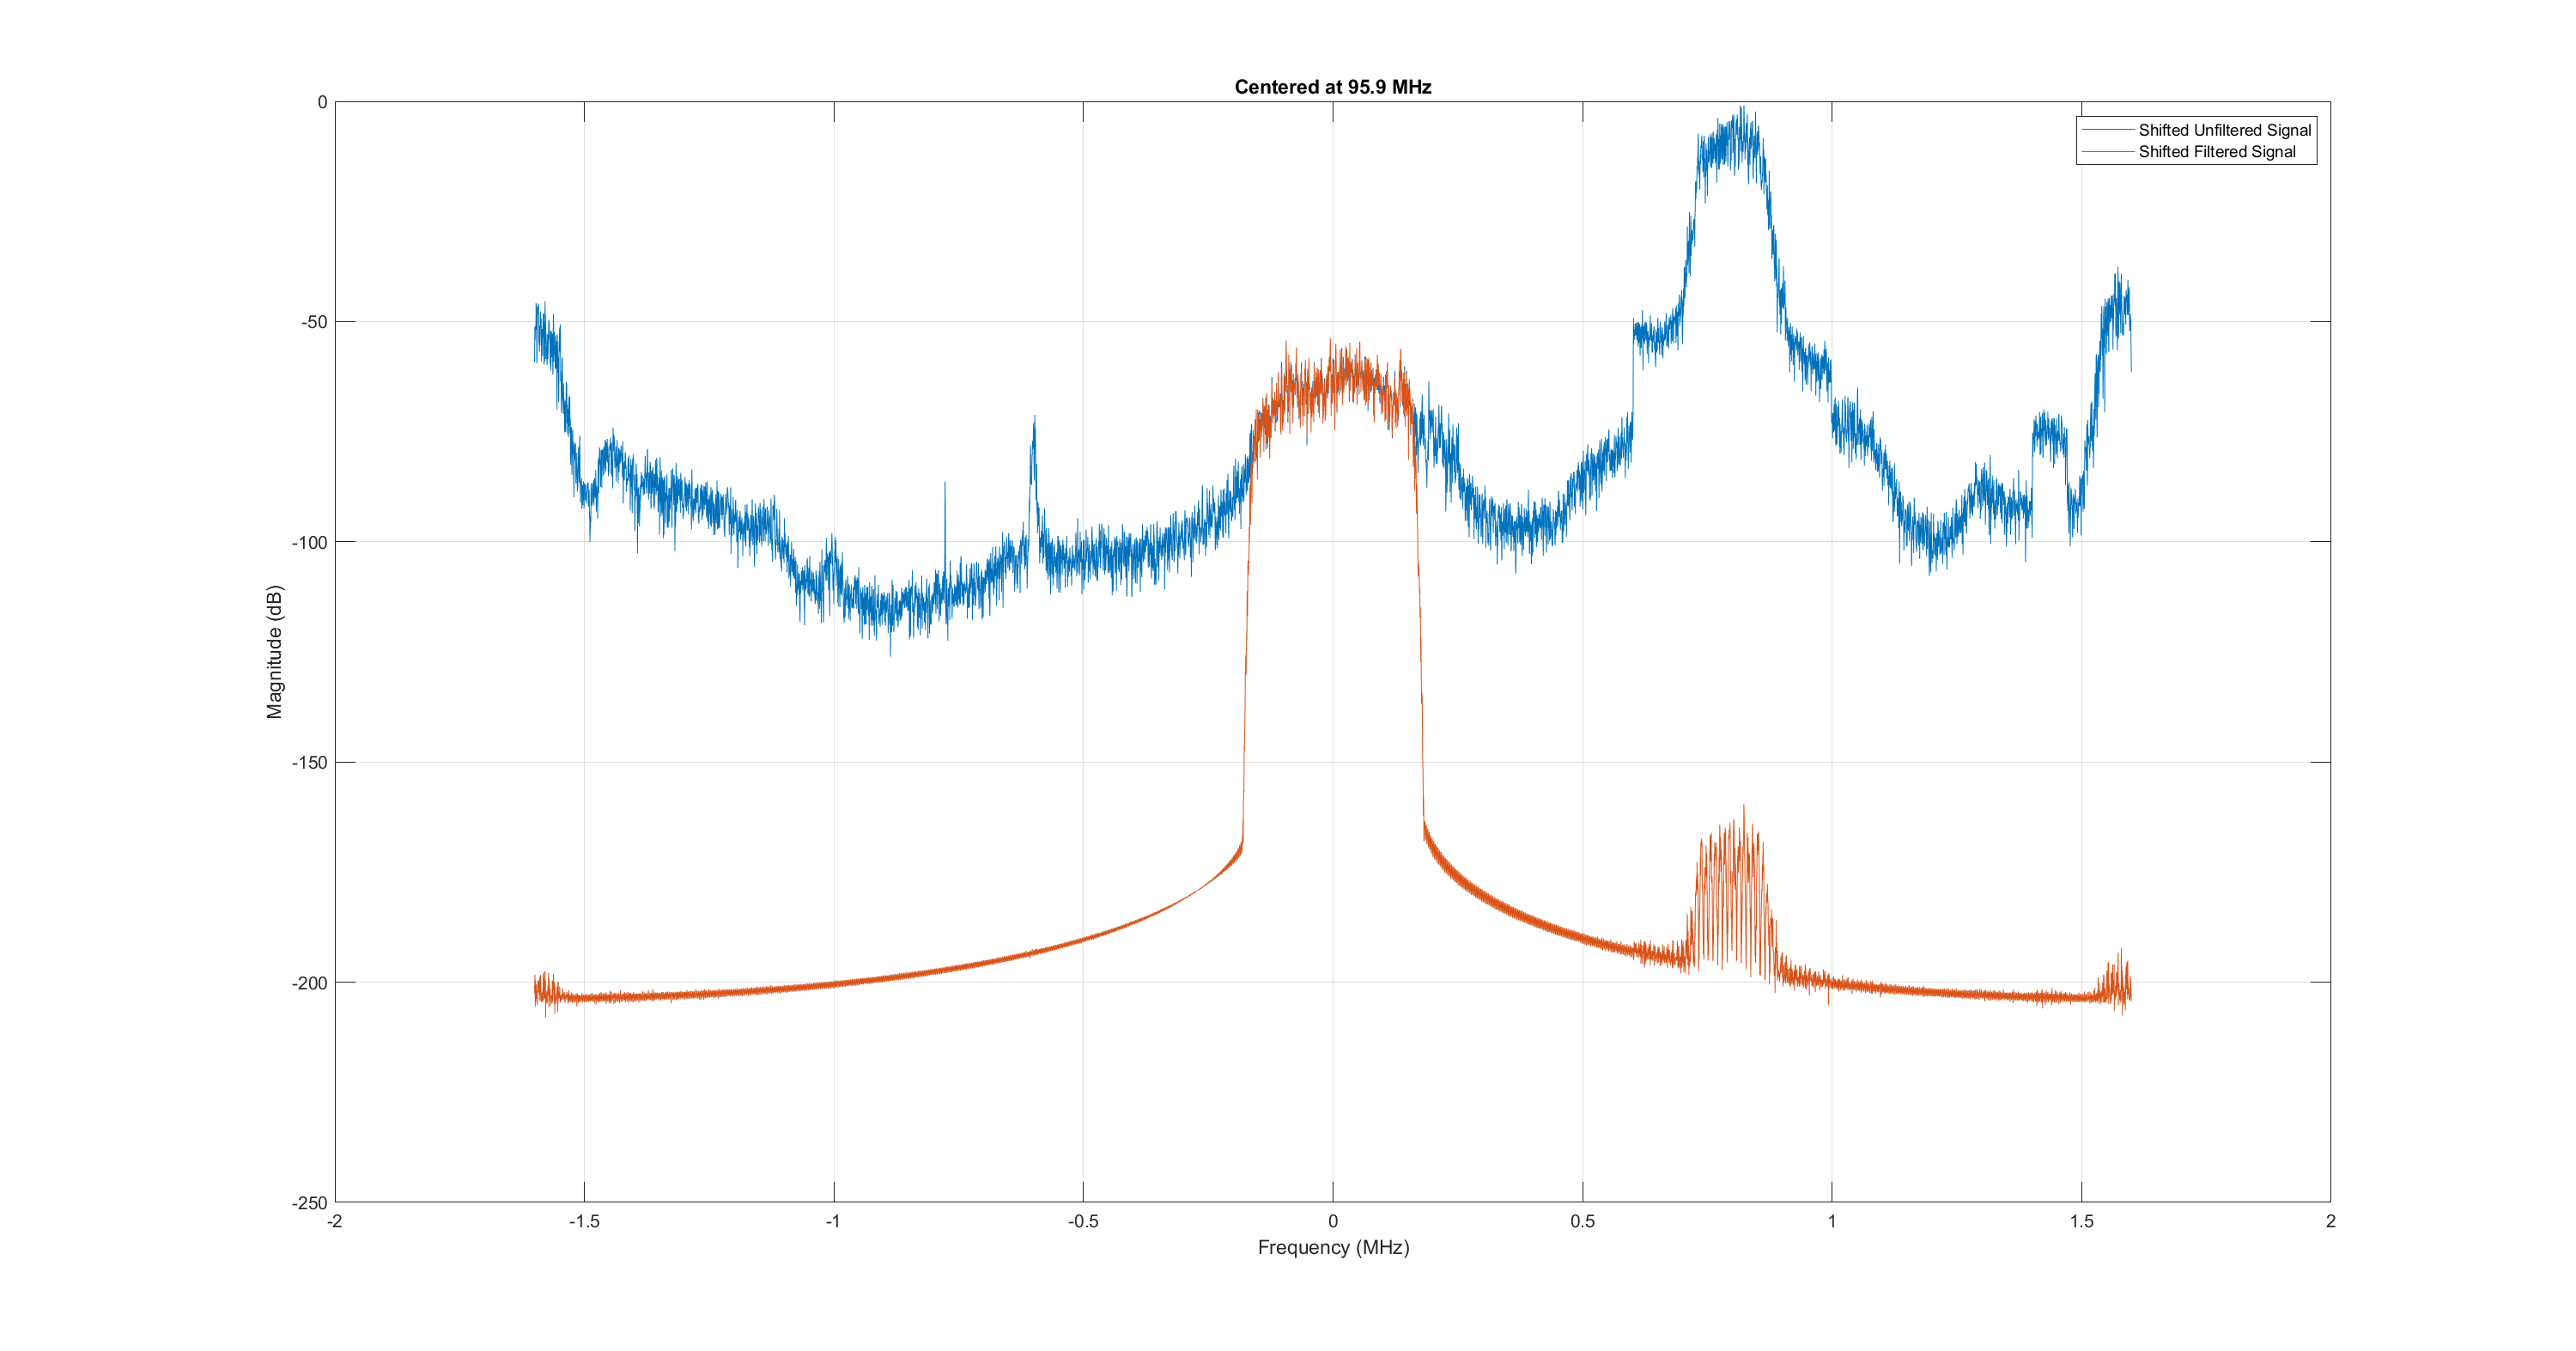
\includegraphics[width=\textwidth]{432_CA2_95.9.png}
        \caption{Centered at 95.9 MHz}
    \end{subfigure}
    
    % Row 3
    \begin{subfigure}[b]{0.23\textwidth}
        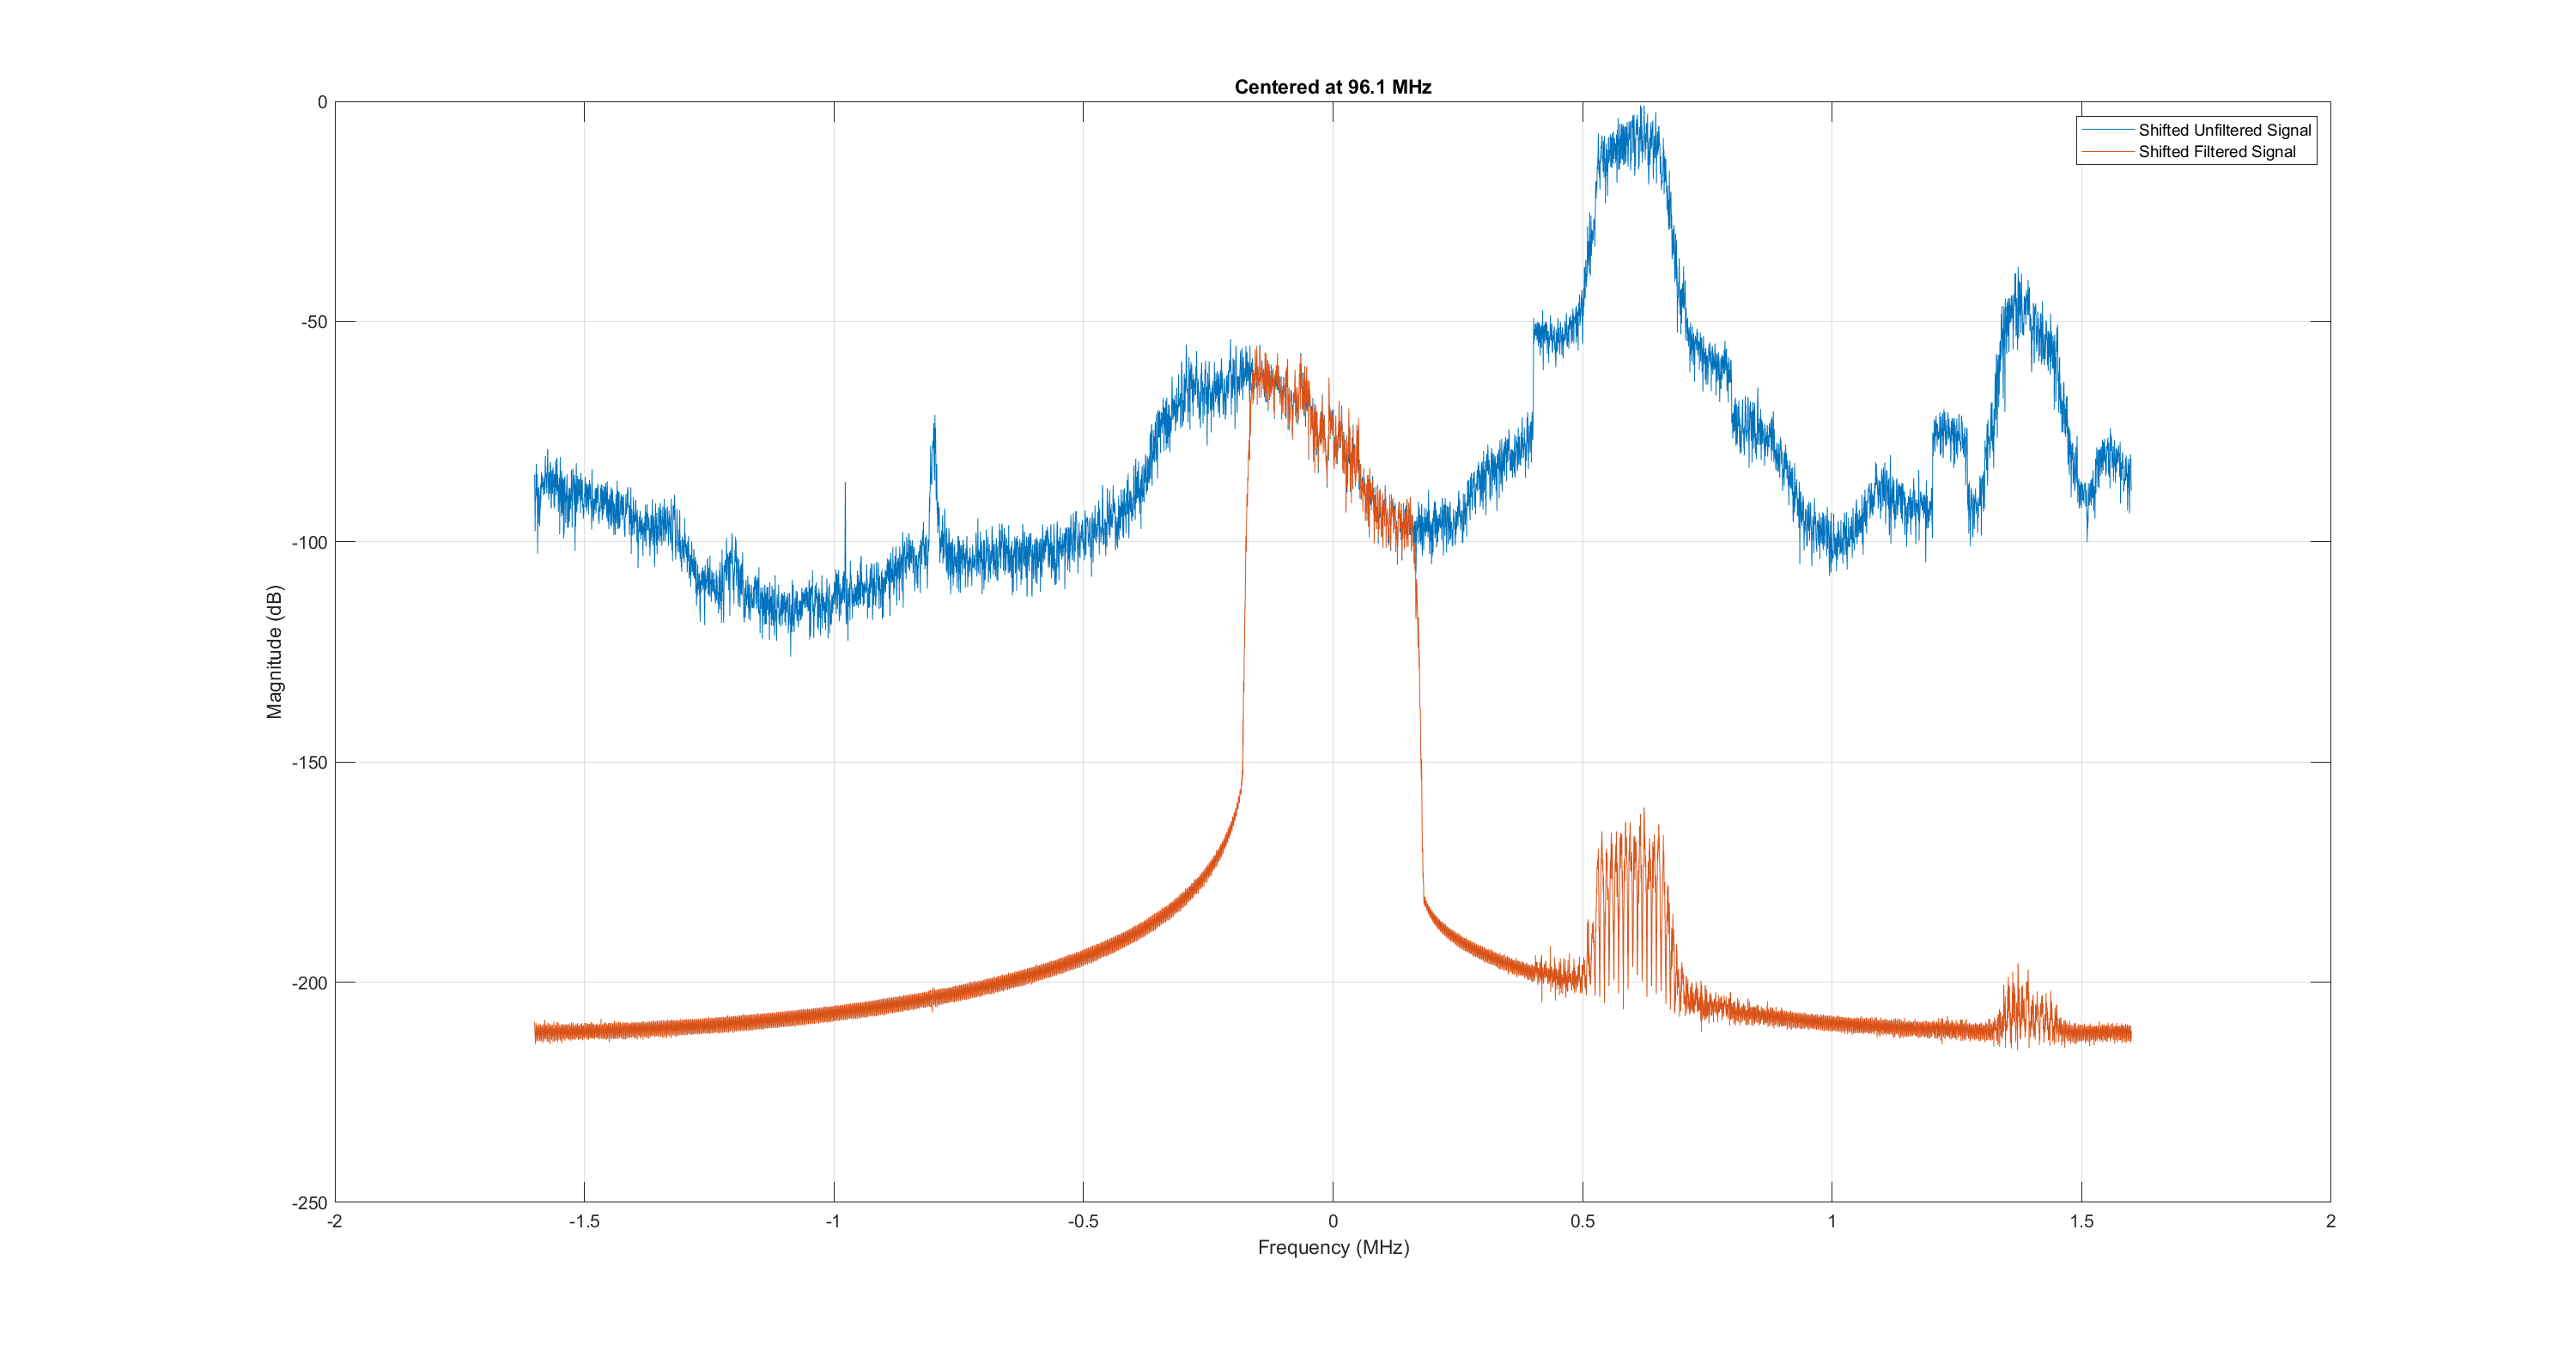
\includegraphics[width=\textwidth]{432_CA2_96.1.png}
        \caption{Centered at 96.1 MHz}
    \end{subfigure}
    \begin{subfigure}[b]{0.23\textwidth}
        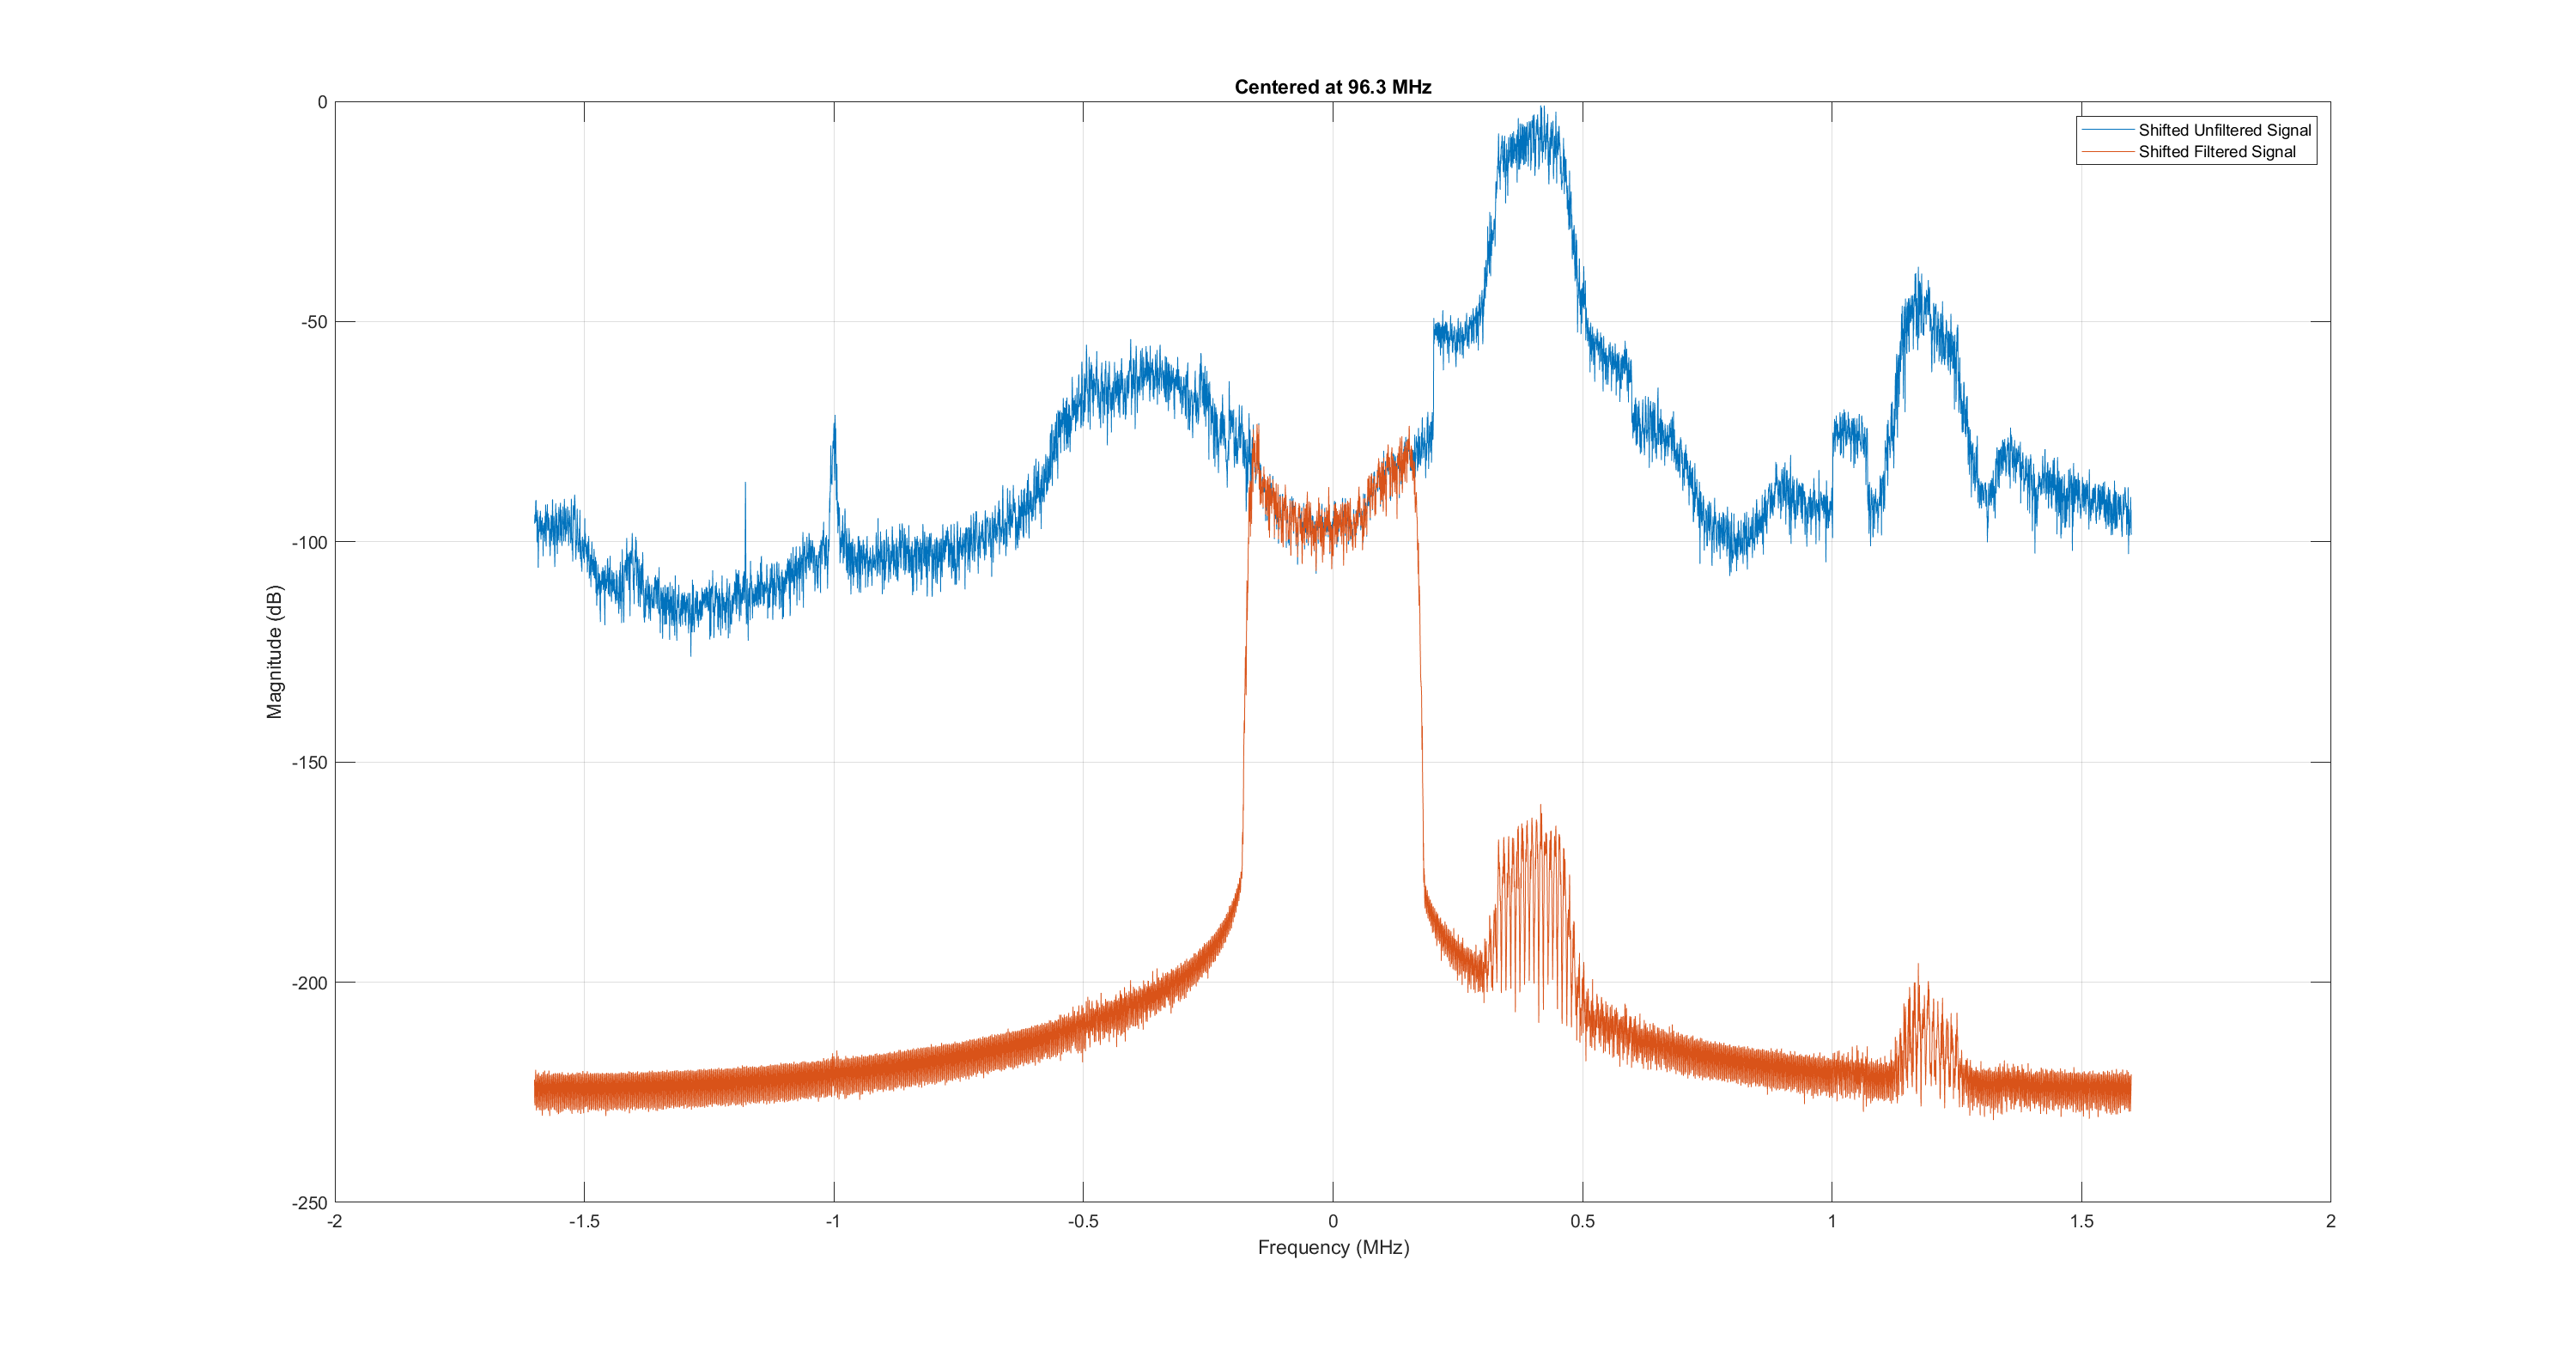
\includegraphics[width=\textwidth]{432_CA2_96.3.png}
        \caption{Centered at 96.3 MHz}
    \end{subfigure}
    \begin{subfigure}[b]{0.23\textwidth}
        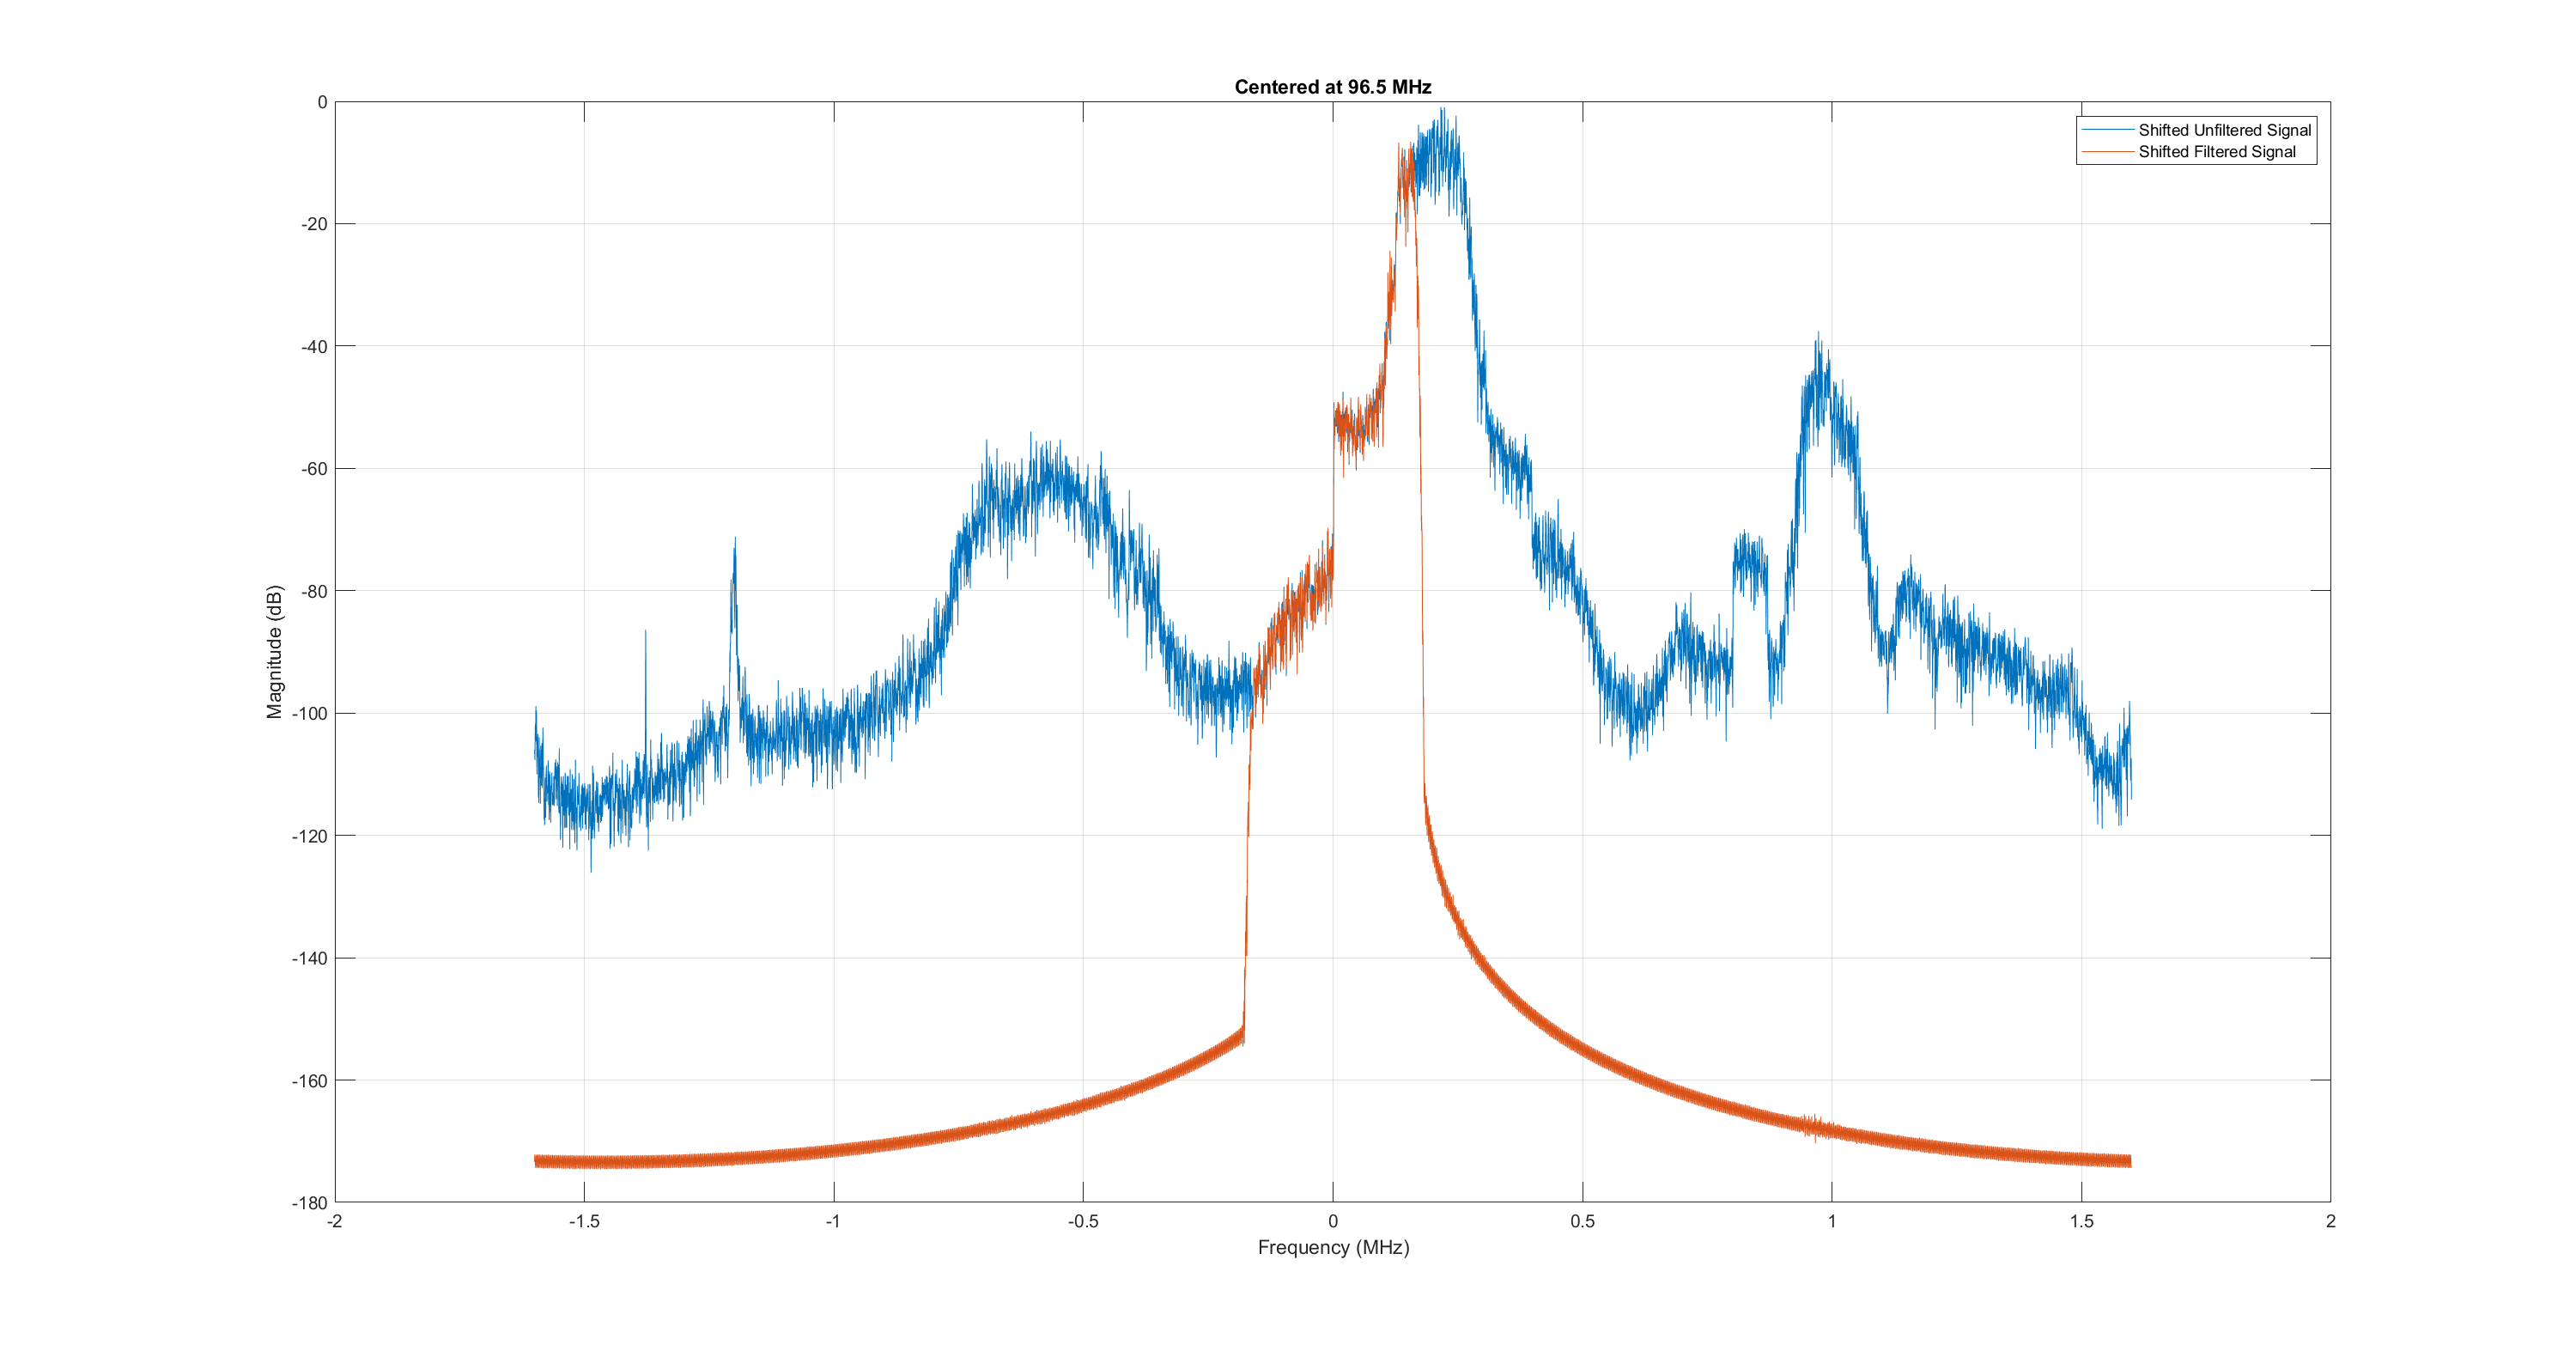
\includegraphics[width=\textwidth]{432_CA2_96.5.png}
        \caption{Centered at 96.5 MHz}
    \end{subfigure}
    \begin{subfigure}[b]{0.23\textwidth}
        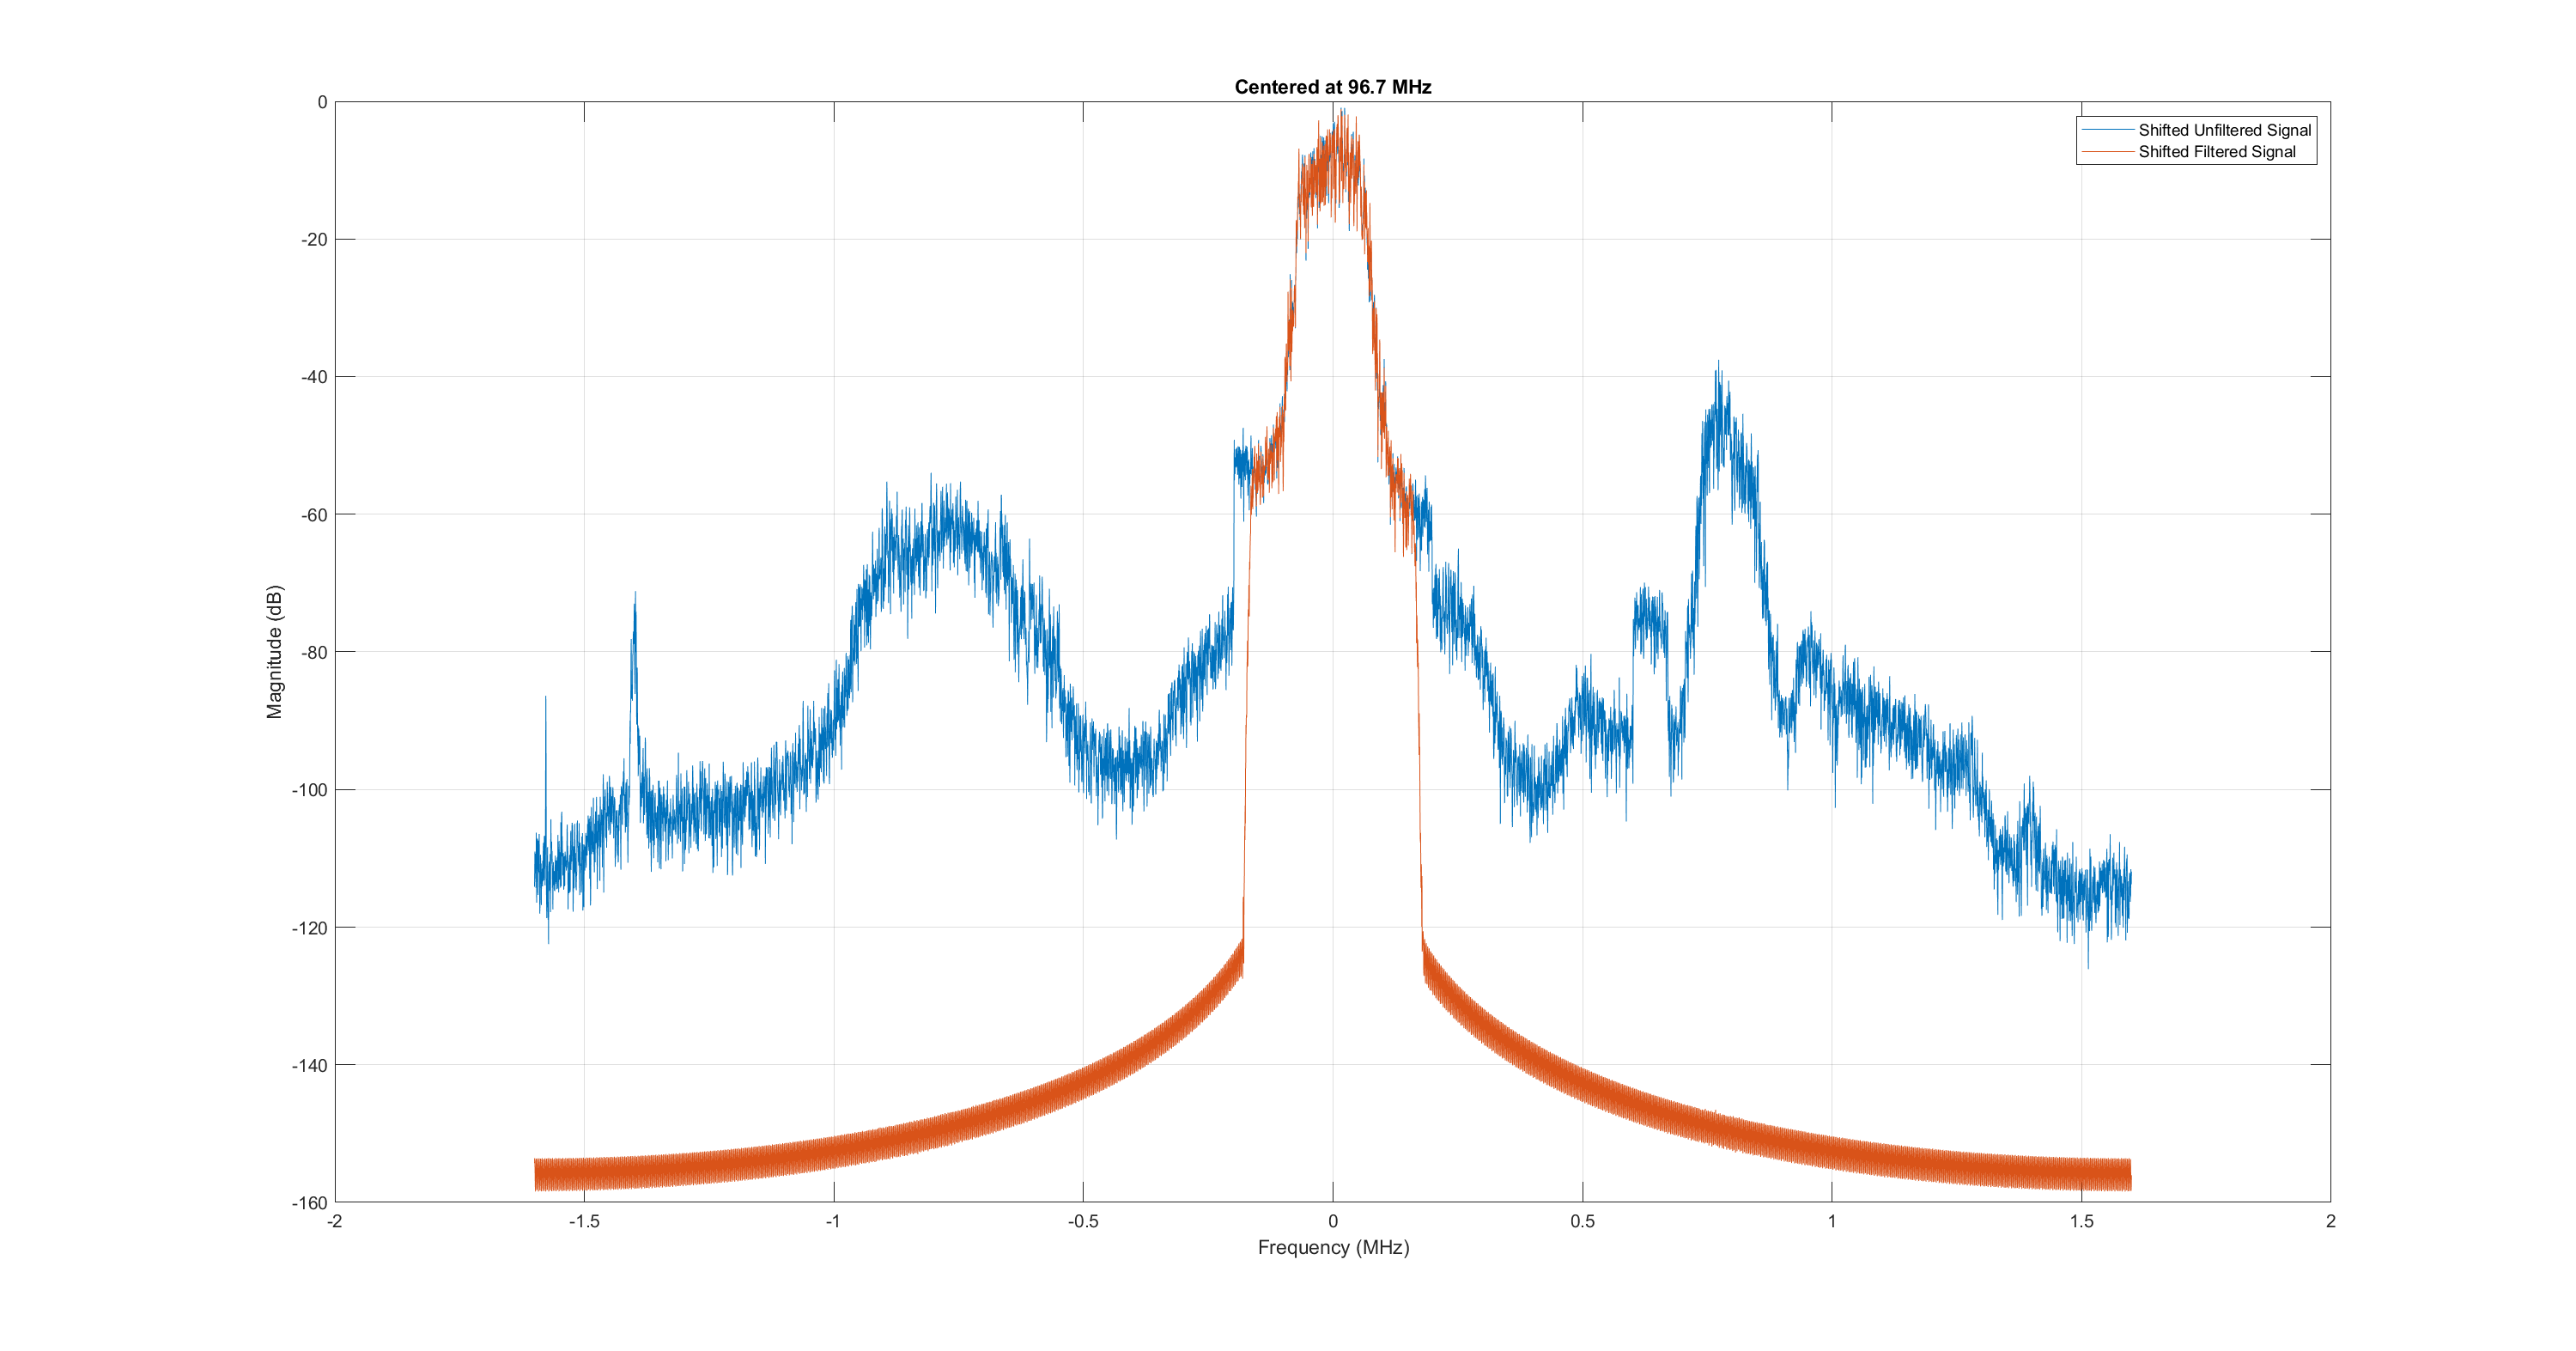
\includegraphics[width=\textwidth]{432_CA2_96.7.png}
        \caption{Centered at 96.7 MHz}
    \end{subfigure}

    % Row 4
    \begin{subfigure}[b]{0.23\textwidth}
        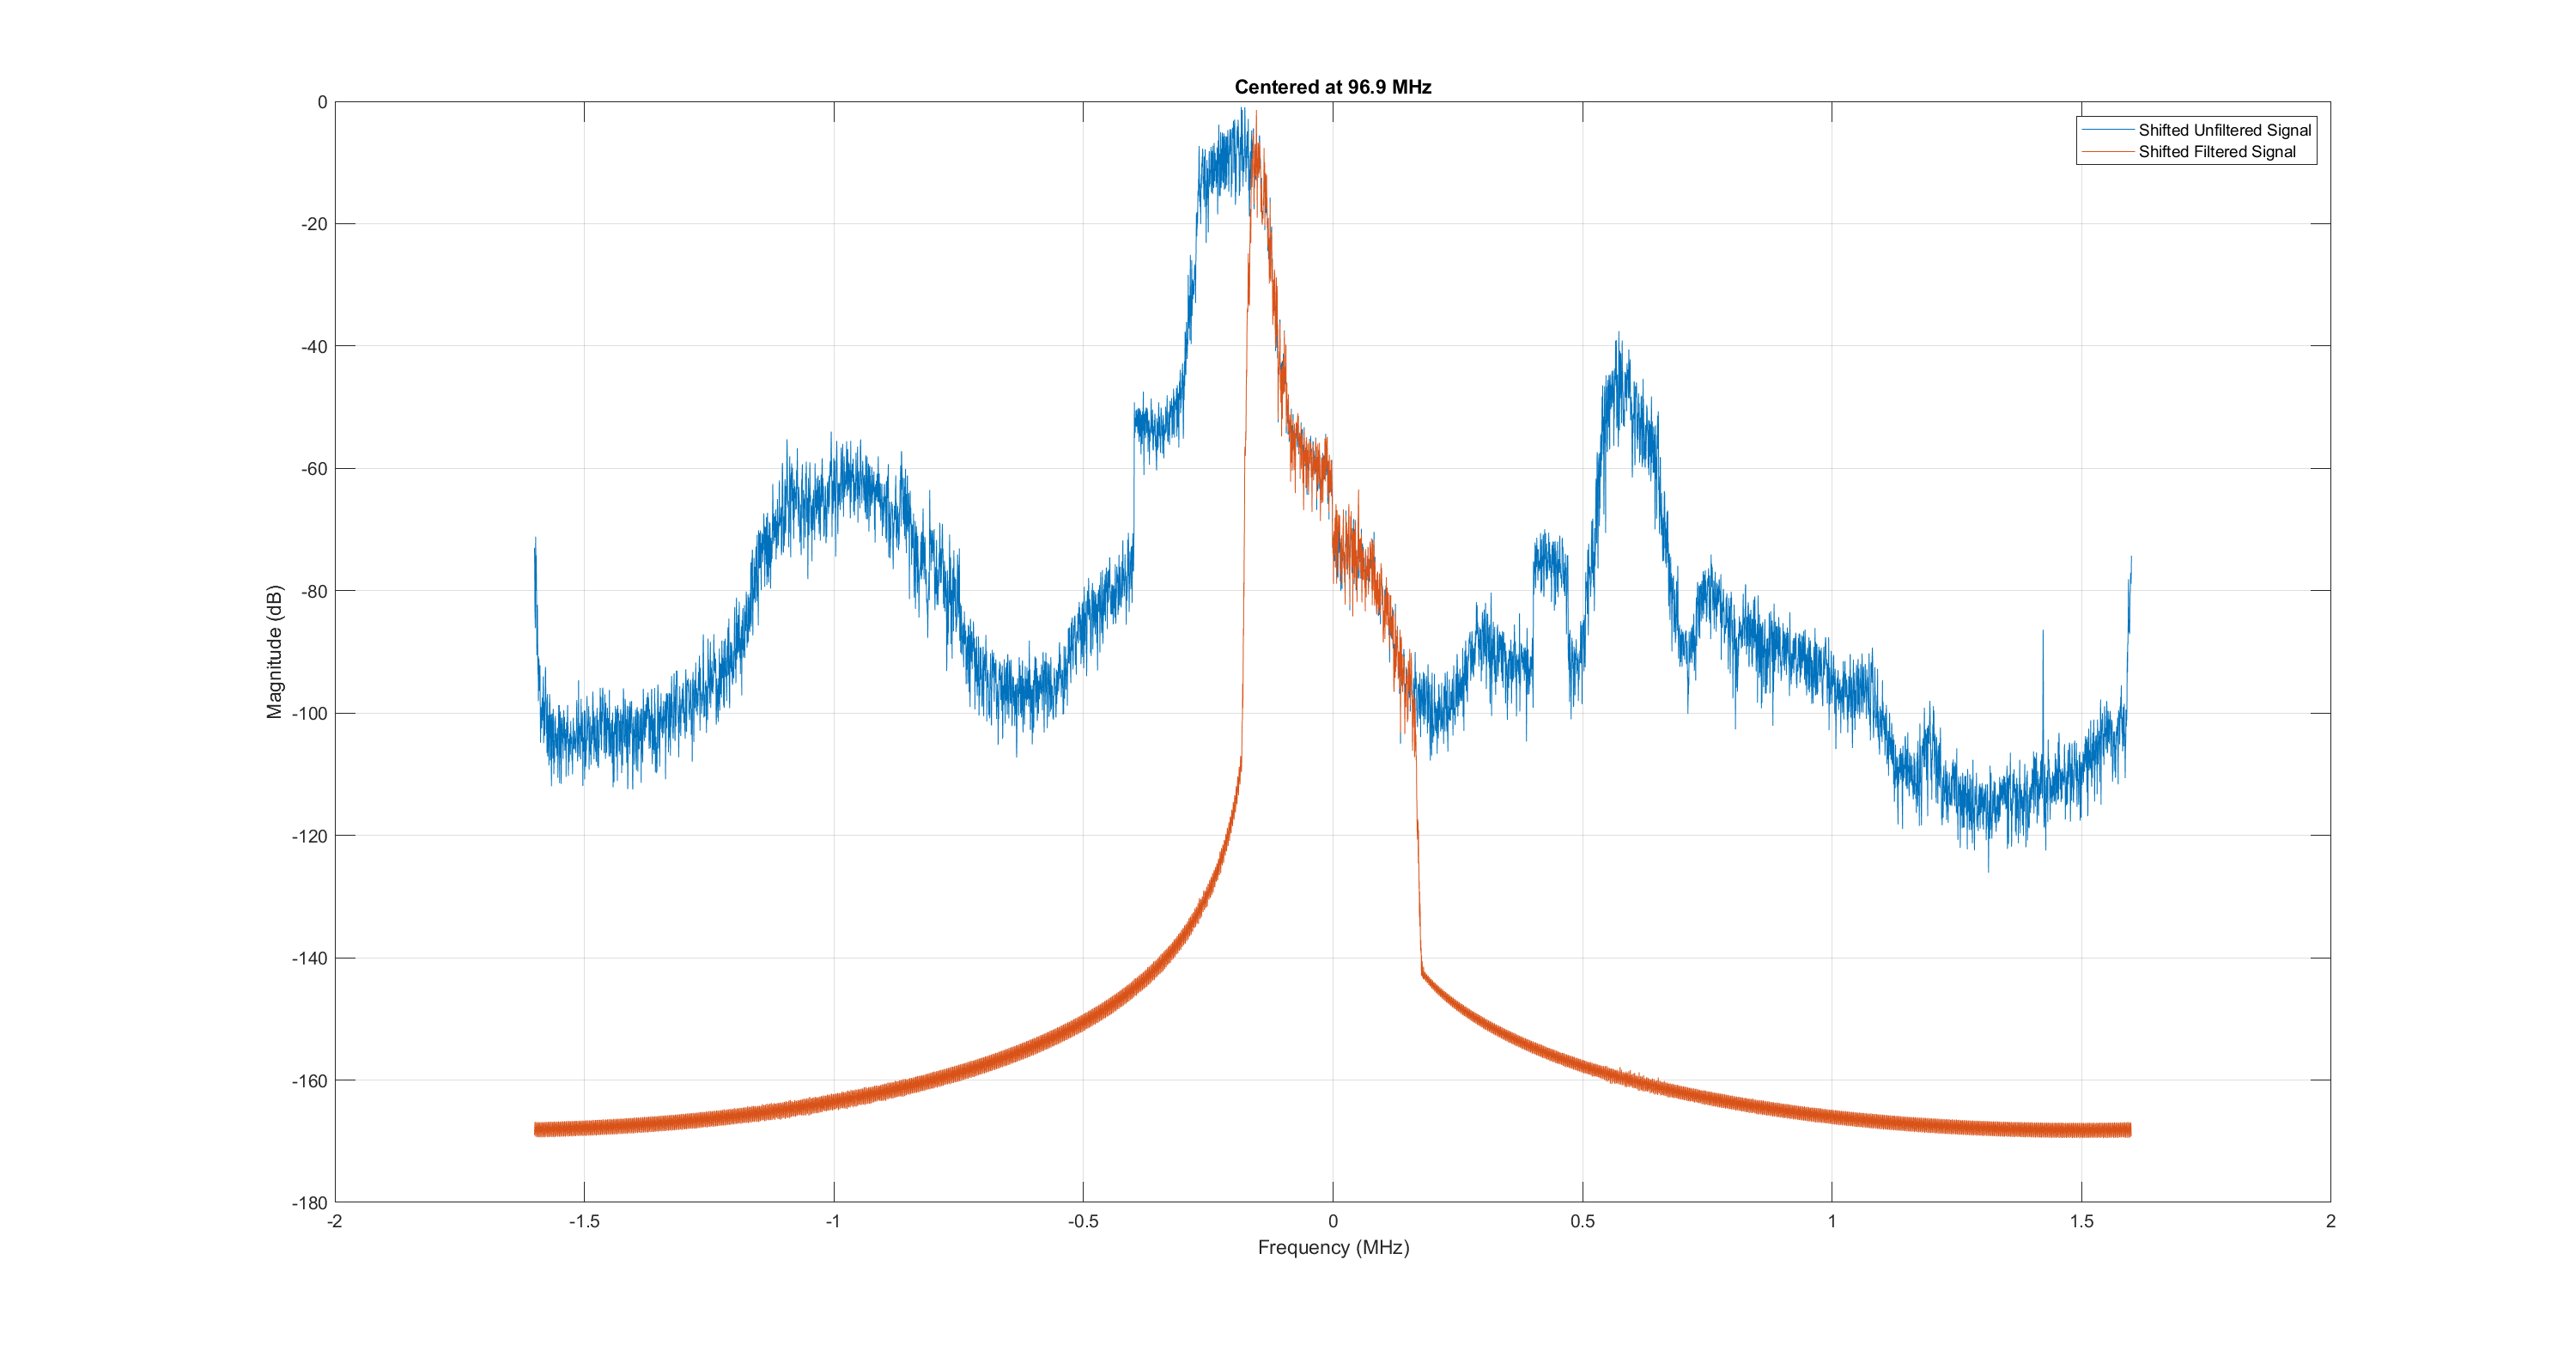
\includegraphics[width=\textwidth]{432_CA2_96.9.png}
        \caption{Centered at 96.9 MHz}
    \end{subfigure}
    \begin{subfigure}[b]{0.23\textwidth}
        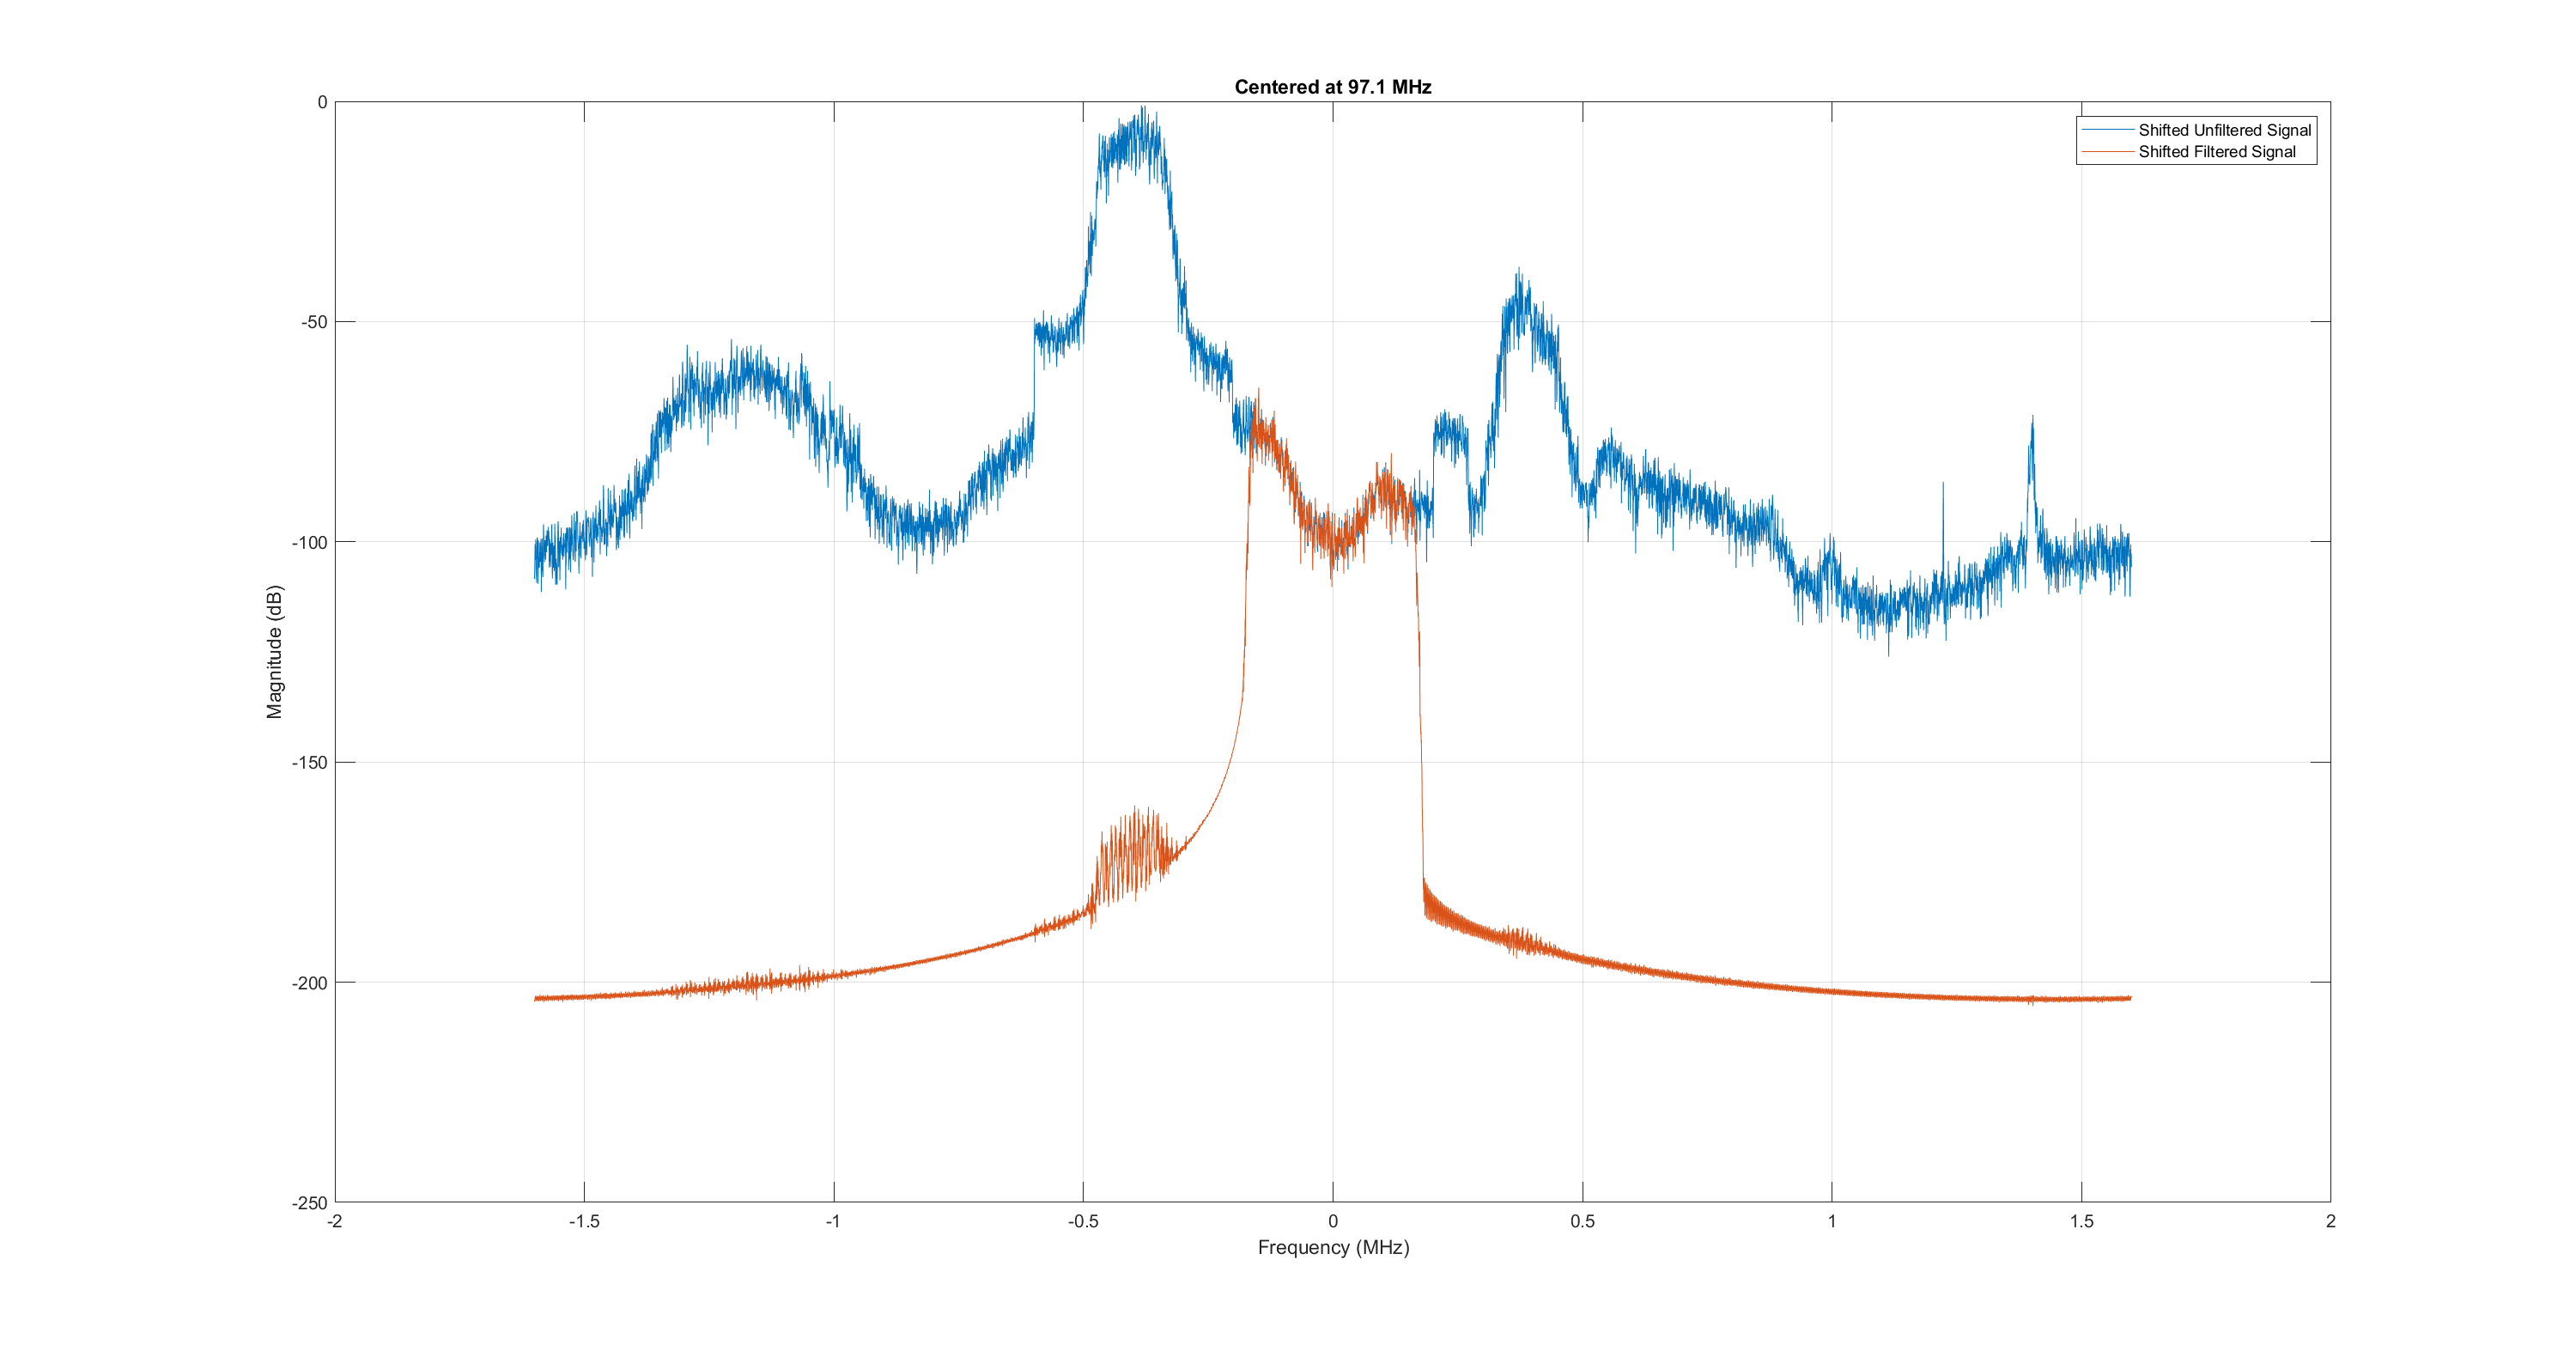
\includegraphics[width=\textwidth]{432_CA2_97.1.png}
        \caption{Centered at 97.1 MHz}
    \end{subfigure}
    \begin{subfigure}[b]{0.23\textwidth}
        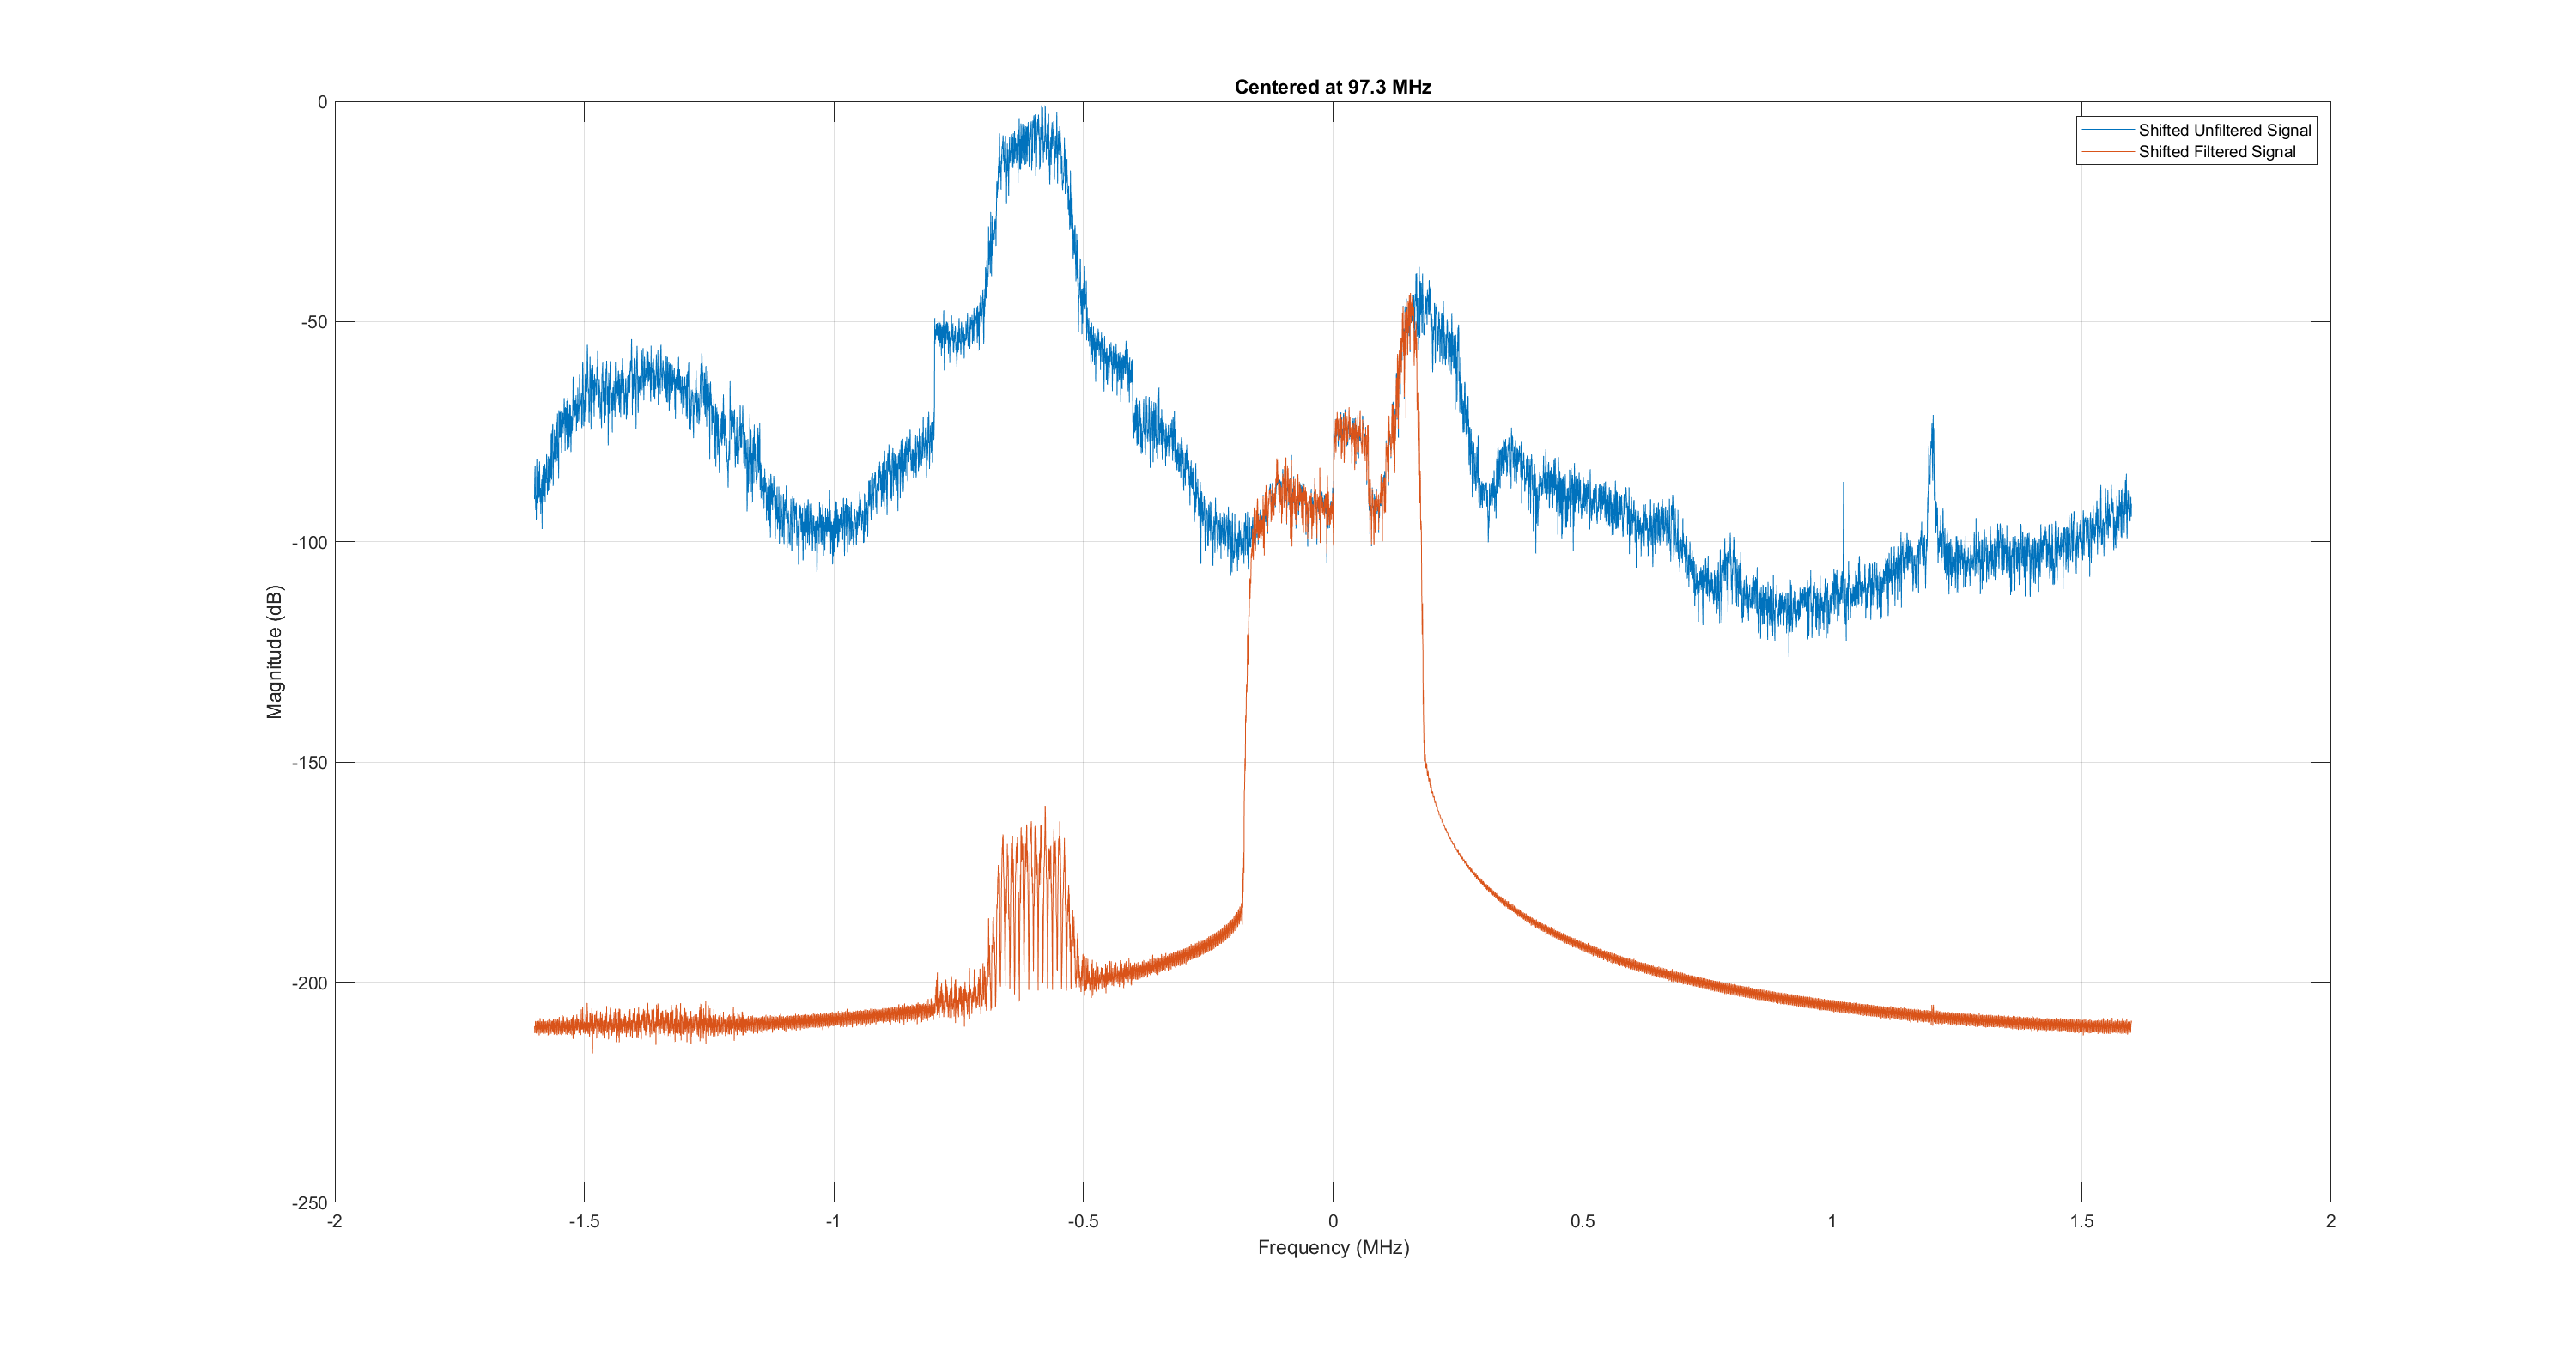
\includegraphics[width=\textwidth]{432_CA2_97.3.png}
        \caption{Centered at 97.3 MHz}
    \end{subfigure}
    \begin{subfigure}[b]{0.23\textwidth}
        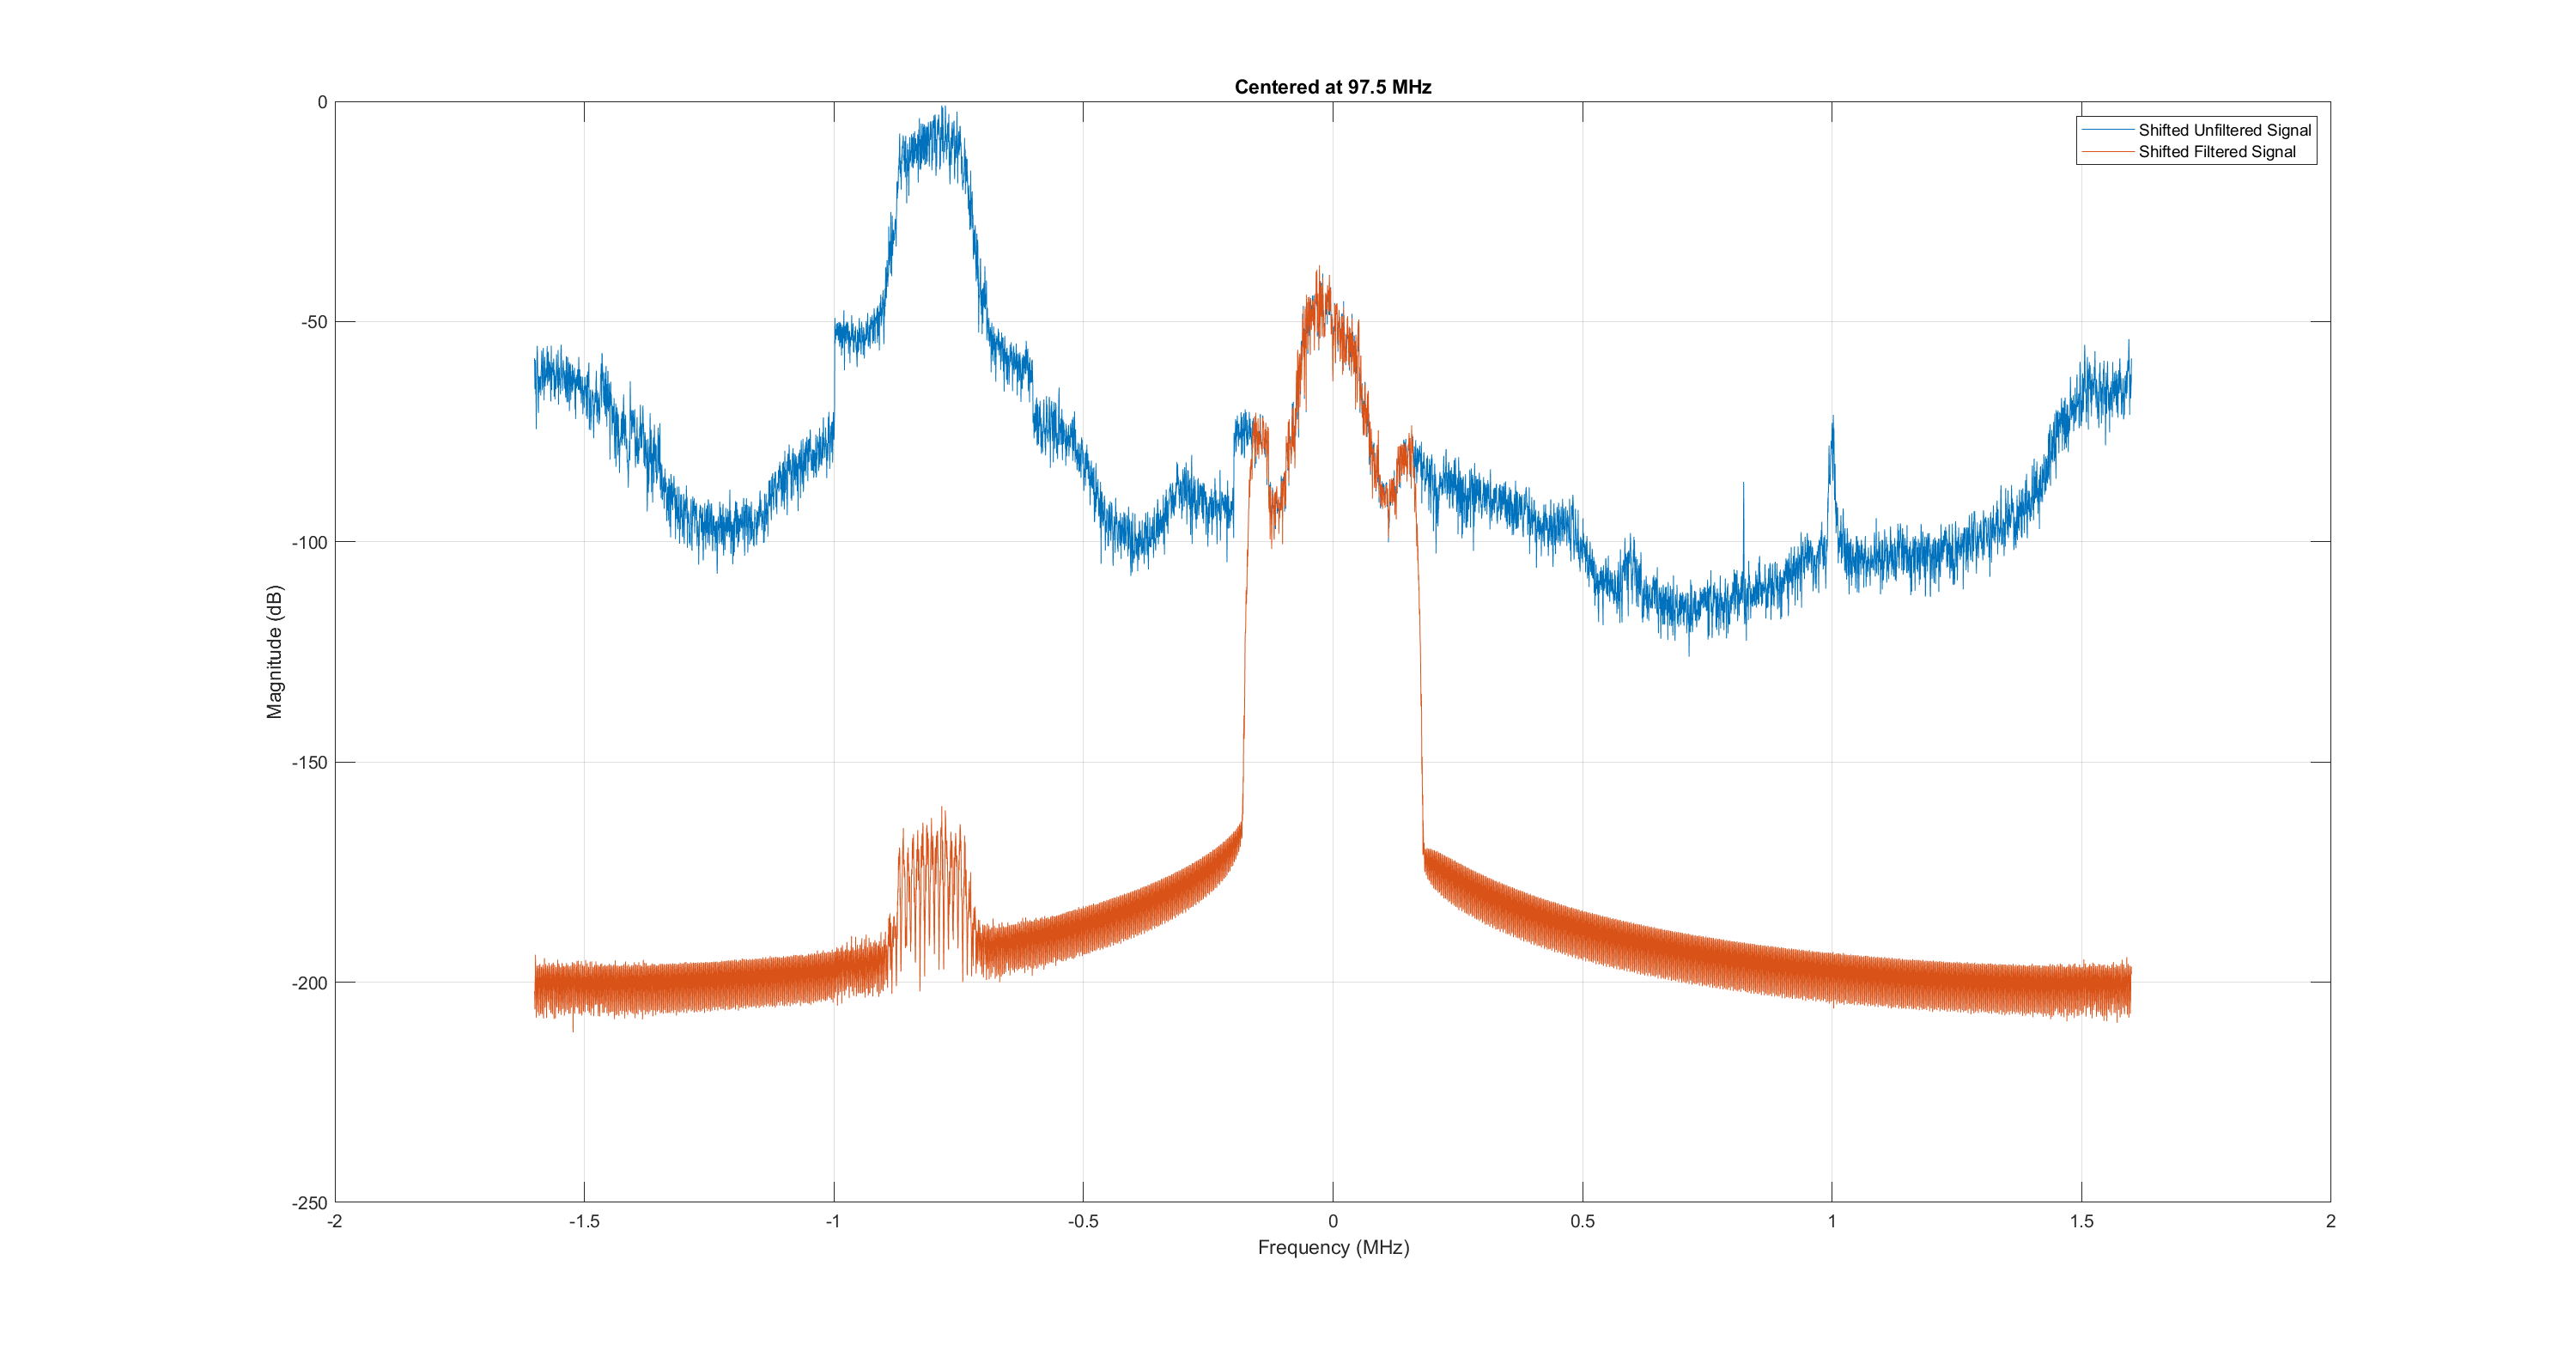
\includegraphics[width=\textwidth]{432_CA2_97.5.png}
        \caption{Centered at 97.5 MHz}
    \end{subfigure}
    
    \caption{Frequency spectrum for various center frequencies between 94.5 MHz and 97.5 MHz.}
    \label{fig:combined}
\end{figure}

\newpage
\begin{figure}[h!]
    \centering
    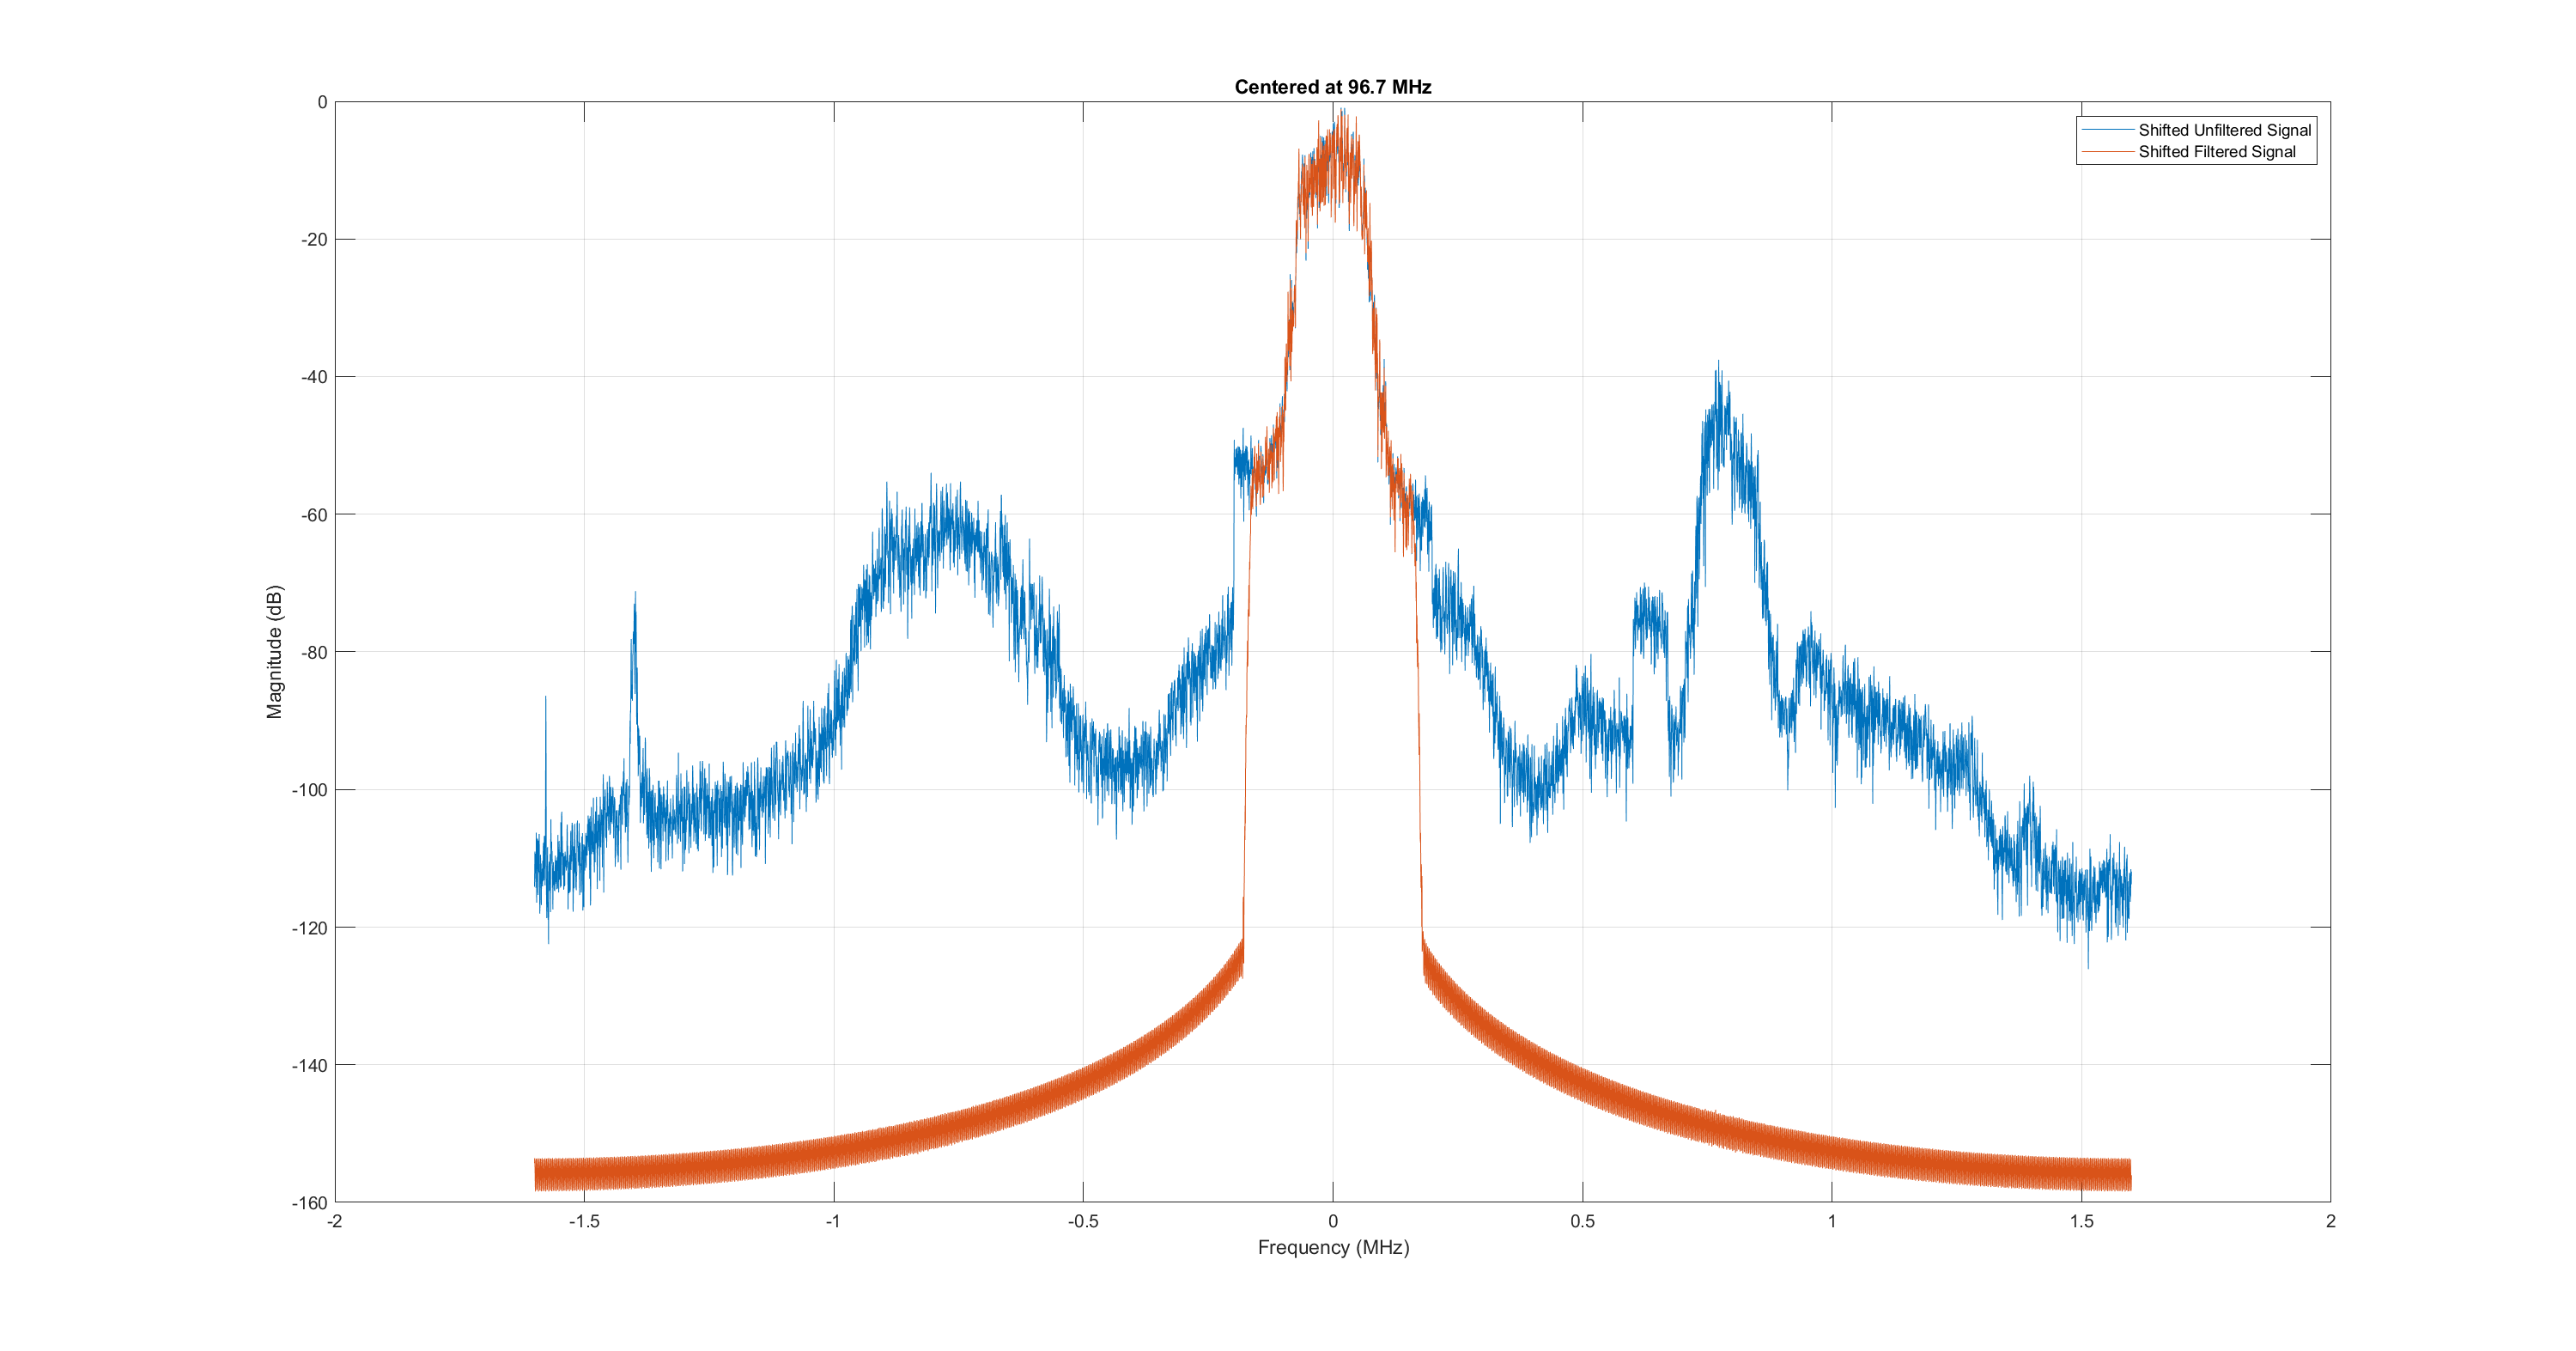
\includegraphics[width=1\textwidth]{432_CA2_96.7.png}
    \caption{Frequency spectrum centered at 96.7 MHz.}
    \label{fig:96.7}
\end{figure}

\begin{figure}[h!]
    \centering
    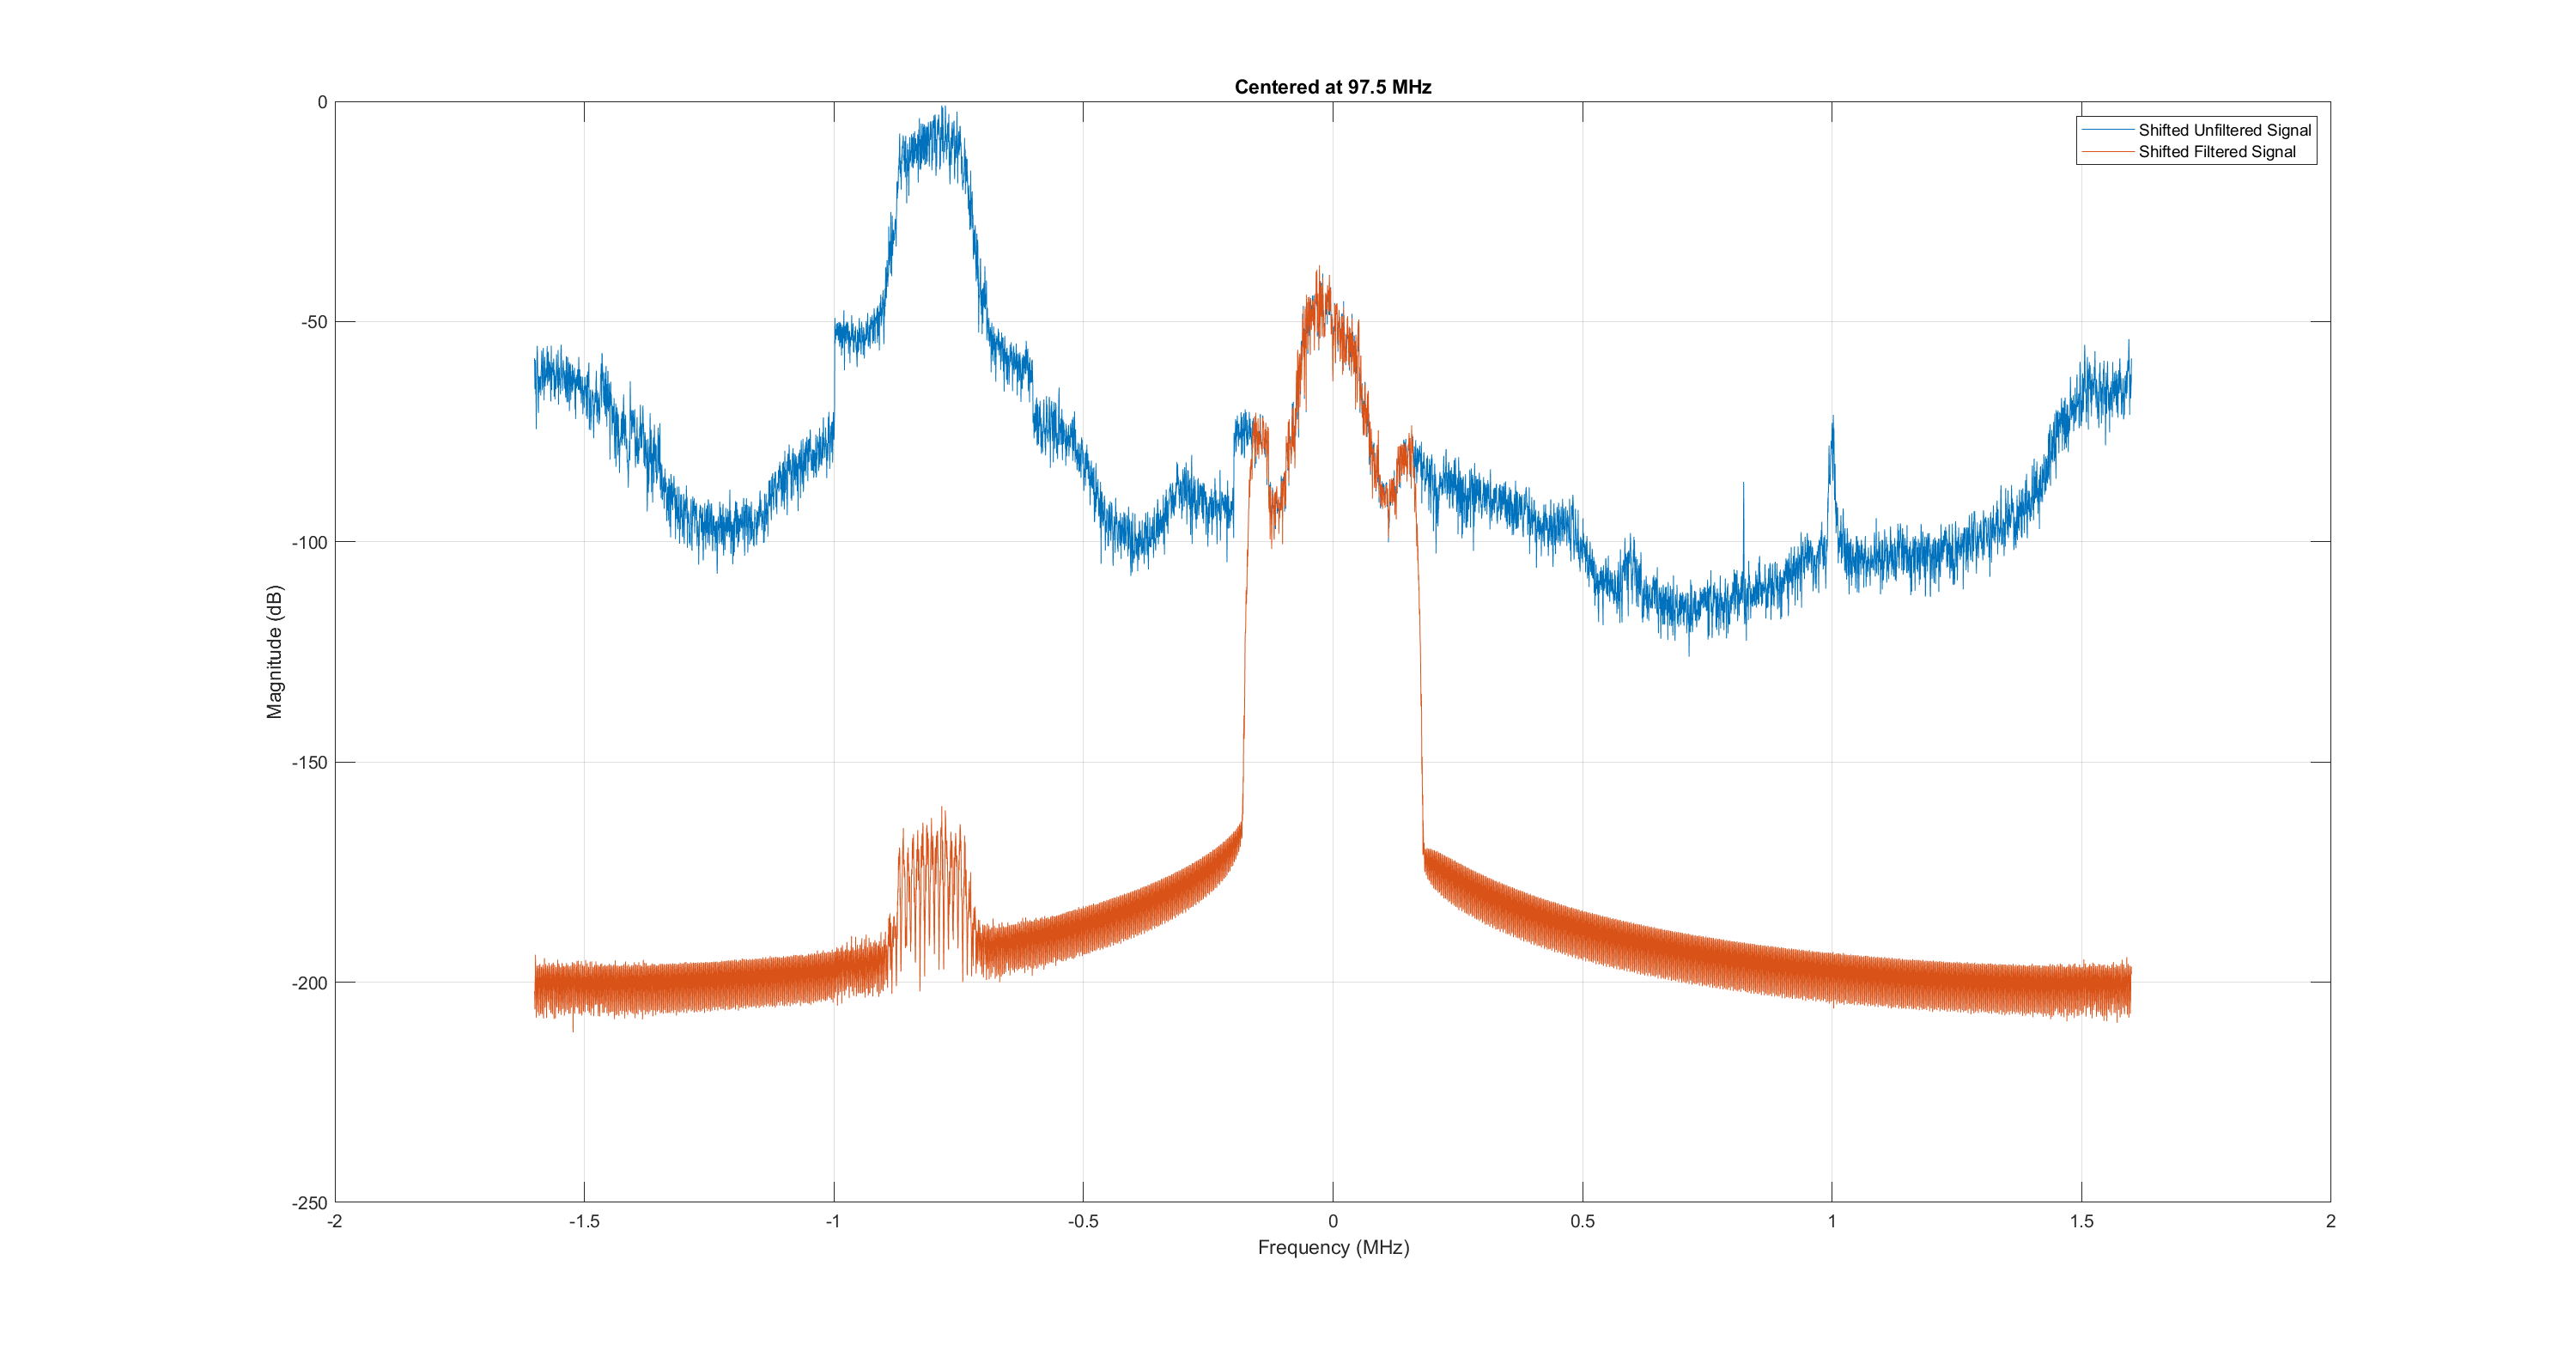
\includegraphics[width=1\textwidth]{432_CA2_97.5.png}
    \caption{Frequency spectrum centered at 97.5 MHz.}
    \label{fig:97.5}
\end{figure}


\newpage % Start a new page for the appendix
\appendix
\section*{MATLAB for generating figures for FM Radio Bands}

The MATLAB code provided performs frequency shifting on a given IQ signal and plots the spectrum for a range of frequencies. The loop iterates through center frequencies from 87.5 MHz to 108.1 MHz, shifting the original IQ signal so that it becomes centered around each of these frequencies.

\begin{verbatim}
clear all
close all
clc

filename = 'SDRSharp_96600000Hz_IQ.wav'; % 1 sec captured IQ data, fs = 3.2 MHz

[data, fs] = audioread(filename);
Tanalysis = 0.01;
Ts = 1/fs;
n = 1:floor(Tanalysis/Ts);
Icomp = data(n, 1);
Qcomp = data(n, 2);

% Loop through frequencies from 87.5 MHz to 108.1 MHz
for f_center = 87.5e6:0.2e6:108.1e6
    % Reload original IQ data
    IQdata = Icomp + 1i * Qcomp;
    
    % Calculate frequency shift
    f_shift = 96.6e6 - f_center;
    
    % Generate complex exponential to shift the frequency
    time_vector = n * Ts;
    complex_exp = exp(-1i * 2 * pi * f_shift * time_vector);
    
    % Shift the signal
    IQdata_shifted = IQdata .* complex_exp';
    
    % Apply your filter (replace with your specific filter function)
    IQdata_filtered = LPfilter(IQdata_shifted);
    
    % Create figure
    figure('Position', [0, 0, 1920, 1080])
    
    [y, h] = pwelch(IQdata_shifted); % power spectral density estimator 
    %for shifted but unfiltered signal
    fspan = (h/2/pi*fs - fs/2)/1e6;
    plot(fspan, 10*log10(abs(fftshift(y)).^2), 'DisplayName', 'Shifted Unfiltered Signal');
    
    hold on
    
    [y, h] = pwelch(IQdata_filtered); % power spectral density %
    estimator for shifted and filtered signal
    fspan = (h/2/pi*fs - fs/2)/1e6;
    plot(fspan, 10*log10(abs(fftshift(y)).^2), 'DisplayName', 'Shifted Filtered Signal');
    
    xlabel('Frequency (MHz)')
    ylabel('Magnitude (dB)')
    grid on
    title(sprintf('Centered at %.1f MHz', f_center / 1e6))
    legend('show')
    
    % Save the figure
    saveas(gcf, sprintf('432_CA2_%.1f.png', f_center / 1e6));
    
    % Close the figure to save memory
    close(gcf);
end
\end{verbatim}
\end{document}
